\documentclass[11pt,reqno]{amsart}
\usepackage[T1]{fontenc}
\usepackage[utf8]{inputenc}
\usepackage{lmodern}
\usepackage[a4paper,margin=27mm]{geometry}
\usepackage{amsmath,amssymb,mathtools,booktabs,array,longtable}
\usepackage{tikz}
\usetikzlibrary{calc,arrows.meta}
\usepackage{microtype}
\usepackage{xurl}
\usepackage[hidelinks]{hyperref}
\hypersetup{pdftitle={Polya's inequality for a square with an arbitrary square hole},pdfauthor={R. Arun Chandru}}
\numberwithin{equation}{section}
\setcounter{tocdepth}{1}
\allowdisplaybreaks[2]
\emergencystretch=2em
\raggedbottom
\newcommand{\R}{\mathbb R}
\newcommand{\N}{\mathbb N}
\newcommand{\Z}{\mathbb Z}
\newcommand{\dd}{\,\mathrm d}
\newcommand{\abs}[1]{\lvert#1\rvert}
\newcommand{\norm}[1]{\lVert#1\rVert}
\newcommand{\Om}{\Omega}
\newcommand{\sstar}{s_*}
\title[P\'olya's inequality for square holes]{P\'olya's inequality for a square\texorpdfstring{\\}{ }with an arbitrary square hole}
\author{R. Arun Chandru}
\email{arun.chandru@gmail.com}
\date{28 September 2026}
\subjclass[2020]{Primary 35P15; Secondary 35P20, 11P21, 33C10, 65G20}
\keywords{P\'olya's conjecture, Dirichlet Laplacian, square hole, perforated domain, mixed boundary conditions, Bessel phase, lattice counting, computer-assisted proof}
\begin{document}
\begin{abstract}
We prove P\'olya's inequality for every Dirichlet eigenvalue of a
Euclidean square with a closed square removed. The hole is contained
in the closed outer square, and the remaining area is positive.
Its feasible size, orientation and position are arbitrary; boundary
contact and disconnected complements are allowed.
Complementary square counts give position-independent spectral
comparisons, while restrictions of low square modes and transport
between actual form domains control the finite spectral range.
For large holes, a mixed-boundary decomposition into sectors and
corners retains the deficit needed at the true area. Conformal
models for the corner caps preserve Dirichlet energy; their mass
weights, endpoint conditions and area costs are explicitly accounted
for. Bessel phase bounds and exact lattice-deficit comparisons cover
the unbounded ranges, including simultaneous small-angle and
small-gap degeneration. Integer and rational certificates handle
closed real parameter intervals, not sampled geometries or approximate
eigenvalues. We also establish the exact total-side threshold for a
universal square-deficit subtraction criterion, yielding a
multiple-hole conclusion, and an independent result for large
parallel rectangular holes with unrestricted displacement.
\end{abstract}
\maketitle
\tableofcontents
\clearpage

\section{Introduction}\label{sec:introduction}

The Dirichlet eigenvalues of a planar domain describe the frequencies
of a membrane fixed along its boundary. Weyl's law determines their
leading density, but does not decide whether the counting function
lies below its leading term at every energy. P\'olya's conjecture asks
for precisely this one-sided statement. For a bounded planar domain
$\Om$, it predicts
\begin{equation}\label{eq:polya}
 |\Om|\lambda_k^D(\Om)\ge4\pi k\qquad(k\in\N),
\end{equation}
where $\N=\{1,2,\ldots\}$ and eigenvalues are repeated according to
multiplicity. The coefficient is fixed by Weyl's law. The challenge is
to keep that exact coefficient through the low spectrum, spectral
clusters, and the entire unbounded energy range.

Perforated domains make the difficulty particularly transparent.
Removing a hole increases each Dirichlet eigenvalue, but decreases
the area multiplying it in \eqref{eq:polya}. Domain monotonicity
alone controls only the first change. Rotation and displacement
leave the isolated spectrum of the hole unchanged while changing
the geometry of the remaining domain. Near boundary contact, some
geometric scales may tend to zero while others remain substantial.
An estimate uniform in these configurations cannot simply use a
remainder whose constant depends on a positive lower boundary gap.

\subsection*{The complete square-hole family}

Let $Q$ be an open square in the Euclidean plane and let $H$ be
a closed square of positive side length contained in $\overline Q$,
with $|Q\setminus H|>0$.
The principal result of this paper is
\begin{equation}\label{eq:main-frame}
 \boxed{\;|Q\setminus H|\lambda_k^D(Q\setminus H)
            \ge4\pi k\quad\hbox{for every }k\in\N.\;}
\end{equation}
The side length, orientation and position of $H$ are arbitrary
subject only to these conditions. In particular, the assertion
includes arbitrary small positive boundary clearances and boundary
contact itself; the remaining domain need not be connected.
The main work treats strictly interior holes uniformly down to
arbitrarily small gaps. A final one-sided approximation then includes
contact configurations using only domain monotonicity and convergence
of the areas, not an assumed continuity theorem for eigenvalues.

A similarity reduces the outer side length to one. Square symmetries
then reduce the relative angle to $0\le\theta\le\pi/4$. If the hole
has side $q$, its axis-aligned bounding box has side
\begin{equation}\label{eq:geometry-normalization}
 b=q\kappa,\qquad \kappa=\cos\theta+\sin\theta,
 \qquad 0<q<1,\quad b\le1.
\end{equation}
Every placement for which $H\subset\overline Q$ is allowed.
The remaining area is $1-q^2$, irrespective of
angle or displacement. The inequality is invariant under
similarities, but not under an arbitrary affine change of
coordinates: the latter changes the Euclidean Laplacian. All
comparisons below retain the actual Euclidean energy or display
explicitly the form to which it is compared.

\begin{figure}[ht]
\centering
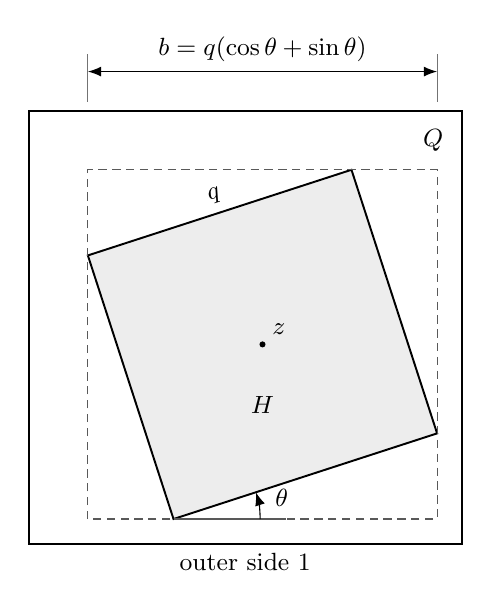
\begin{tikzpicture}[x=5.5cm,y=5.5cm,>=Latex,font=\small]
 \def\qh{0.64}\def\ang{18}\def\cx{0.54}\def\cy{0.46}
 \pgfmathsetmacro{\bh}{\qh*(cos(\ang)+sin(\ang))}
 \coordinate (A) at ({\cx-\qh*cos(\ang)/2+\qh*sin(\ang)/2},
                     {\cy-\qh*sin(\ang)/2-\qh*cos(\ang)/2});
 \coordinate (B) at ({\cx+\qh*cos(\ang)/2+\qh*sin(\ang)/2},
                     {\cy+\qh*sin(\ang)/2-\qh*cos(\ang)/2});
 \coordinate (C) at ({\cx+\qh*cos(\ang)/2-\qh*sin(\ang)/2},
                     {\cy+\qh*sin(\ang)/2+\qh*cos(\ang)/2});
 \coordinate (D) at ({\cx-\qh*cos(\ang)/2-\qh*sin(\ang)/2},
                     {\cy-\qh*sin(\ang)/2+\qh*cos(\ang)/2});
 \draw[line width=.7pt] (0,0) rectangle (1,1);
 \filldraw[fill=black!7,line width=.7pt] (A)--(B)--(C)--(D)--cycle;
 \draw[densely dashed,black!65] ({\cx-\bh/2},{\cy-\bh/2})
                          rectangle ({\cx+\bh/2},{\cy+\bh/2});
 \fill (\cx,\cy) circle[radius=.007];
 \node[above right] at (\cx,\cy) {$z$};
 \node at (\cx,{\cy-.14}) {$H$};
  \node[below left] at (.98,.98) {$Q$};
 \draw[black!65] (A)--++(.26,0);
 \draw[->] ($(A)+(.20,0)$) arc[start angle=0,end angle=\ang,radius=.20];
 \node at ($(A)+(.25,.048)$) {$\theta$};
 \node[above,rotate=18] at ($(C)!.5!(D)$) {$q$};
 \draw[black!55] ({\cx-\bh/2},1.02)--({\cx-\bh/2},1.13);
 \draw[black!55] ({\cx+\bh/2},1.02)--({\cx+\bh/2},1.13);
 \draw[<->] ({\cx-\bh/2},1.09)--node[above]
              {$b=q(\cos\theta+\sin\theta)$}({\cx+\bh/2},1.09);
 \node[below] at (.5,0) {outer side $1$};
\end{tikzpicture}
\caption{A displaced and rotated square hole. The dashed square is
its axis-parallel bounding box, not a boundary of the Dirichlet
domain. The illustrated configuration has positive clearance;
the theorem also permits boundary contact. Solid boundaries carry
Dirichlet conditions.}
\label{fig:square-geometry}
\end{figure}

The inclusive count
$N_\Om(E)=\#\{k:\lambda_k^D(\Om)\le E\}$ gives the equivalent
formulation
\begin{equation}\label{eq:main-count}
 N_{Q\setminus H}(E)\le\frac{|Q\setminus H|}{4\pi}E
 \qquad(E\ge0).
\end{equation}
Multiplicity and endpoint conventions matter in passing between
these two formulations. Our finite-index arguments retain a strict
outer square count and an inclusive hole count. Their conclusions
are used as indexed eigenvalue bounds, without incorrectly turning
an equality at a spectral endpoint into an empty eigenspace.

\subsection*{Two complementary geometric conclusions}

There is also a result for finitely many closed square holes $H_i$
contained in the closure of an outer square of side $L$, with
pairwise disjoint interiors. Outer-boundary and mutual contact are
allowed.
Let their side lengths be $l_i$, with independent positions and
orientations. Put
\begin{equation}\label{eq:sharp-constant}
 s_*=\sqrt{1-\frac{12}{5\pi}}
      =0.485856226839692\ldots.
\end{equation}
Then
\begin{equation}\label{eq:main-holes}
 \sum_i l_i\le s_*L
 \quad\Longrightarrow\quad
 \left|Q\setminus\bigcup_iH_i\right|
 \lambda_k^D\!\left(Q\setminus\bigcup_iH_i\right)\ge4\pi k
 \quad(k\in\N).
\end{equation}
The hypothesis is a sum of side lengths, not a sum of areas.
The sharpness assertion concerns its scalar comparison, not an
optimal restriction on the geometry. More precisely, with
\begin{equation}\label{eq:count-intro}
 C(t)=\#\{(m,n)\in\N^2:m^2+n^2\le t^2\},\qquad
 d(t)=\frac\pi4t^2-C(t),
\end{equation}
we prove
\begin{equation}\label{eq:scalar-main}
 \sum_i d(q_it)\le d(t)
 \qquad\left(q_i\ge0,\ \sum_iq_i\le s_*,\ t\ge0\right),
\end{equation}
and show that no larger total-side threshold guarantees this
inequality for all finite lists. The complete one-hole conclusion
\eqref{eq:main-frame} goes beyond this scalar criterion.

Finally, let a single parallel rectangular hole have side lengths
$pL,qL$ and arbitrary strictly interior position. We prove
\begin{equation}\label{eq:main-displaced}
 \frac{11}{12}\le p,q<1
 \quad\Longrightarrow\quad
 |Q\setminus H|\lambda_k^D(Q\setminus H)\ge4\pi k
 \quad(k\in\N).
\end{equation}
The two side ratios and the individual boundary gaps vary
independently. This conclusion is not obtained by stretching
\eqref{eq:main-frame}; its proof uses a separate two-scale
mixed-boundary comparison. The sufficient constant $11/12$ is not
asserted optimal.

\subsection*{Prior work and the contribution here}

P\'olya proved the conjectured inequality for tiling planar domains
\cite{Polya1961}. The inequalities of Berezin and Li--Yau control
eigenvalue averages \cite{Berezin1972,LiYau1983}; these do not
directly give the conjectured coefficient at each individual index.
Product constructions, unions and packing arguments supply further
classes and reductions \cite{Laptev1997,FLP2021,FS2023,HW2026}.
Filonov, Levitin, Polterovich and Sher proved P\'olya's conjecture
for Euclidean balls \cite{FLPS2023} and its Dirichlet form for
planar circular annuli \cite{FLPS2026}. The annulus proof combines
variational estimates, Bessel analysis, lattice counting and
rigorous finite computation. Neither topological equivalence nor
conformal equivalence transfers that spectral conclusion to the
polygonal domains studied here: conformal change preserves planar
Dirichlet energy, but changes the mass in the Rayleigh quotient.

Jiang and Lin develop complementary counting comparisons for
perforated strip-tiling domains, as well as explicit estimates with
an $\epsilon$-loss for general Lipschitz domains \cite{JL2026}.
For square holes in a square, their Theorem~1.15 gives the
sufficient total-side condition
$\sum_i l_i/L\le1/(2\sqrt2\pi)$. The variational subtraction
principle is an established input here, not a new abstract
monotonicity theorem. Our multiple-hole contribution is the exact
threshold \eqref{eq:sharp-constant} for the stated universal
square-deficit comparison, including its finite-list aggregation.

The principal geometric contribution is the full family
\eqref{eq:main-frame}. Its proof must keep three types of
information together. Complementary square spectra provide
position-independent arithmetic bounds. Low-mode restriction and
actual-domain transport retain geometric information where those
bounds are insufficient. In the near-filling regime, the true-area
deficit from four mixed sectors pays for the corner comparison
costs. The circular cap models used in this last step have
explicitly tracked mass weights and singular endpoint domains;
their counts are not substituted for the original count without
a form comparison. Horsley's Bessel derivative-phase estimates
\cite{Horsley2017} supply a global radial input, with the
first-eigenvalue indexing handled explicitly below.

The disk estimates used in the arithmetic part are elementary
Poisson--Bessel bounds with constants chosen for the finite
verification. They are not claims to a new Gauss-circle discrepancy
record. Likewise, the computer-assisted steps do not calculate
approximate eigenvalues of a perforated square. They certify
integer and rational inequalities on closed parameter intervals,
after analysis has bounded the remaining spectral range.
Classical Weyl asymptotics and more recent remainder and
Riesz-mean results provide important context
\cite{Weyl1912,JL2026,FrankLarson2025}, but are not used as a
replacement for an all-energy proof with the exact coefficient.

\subsection*{How the argument fits together}

We first fix the variational and counting conventions
and prove the scalar aggregation for small holes. The next part
develops the low-mode and transport comparisons for rotated holes.
Elementary one-dimensional sums then support the mixed-sector and
corner analysis for large holes. The arithmetic section proves the
explicit disk estimate, its paired-deficit refinements and the
finite-index cover, bringing these arguments together for every
strictly interior square hole. One-sided approximation then includes
boundary contact. The independent rectangular-hole comparison follows.
The appendices specify the additional finite certificates
for the multiple-hole and rectangular conclusions.


\section{The Dirichlet form and complementary square counts}\label{sec:comparison}

We begin with strictly interior, pairwise disjoint holes. These
domains are bounded and polygonal, with finitely many separated
boundary components. Their Dirichlet Laplacian is
the selfadjoint operator associated with
\[
 \mathfrak a_\Om[u]=\int_\Om|\nabla u|^2\dd x,
 \qquad u\in H^1_0(\Om),
\]
in $L^2(\Om)$. The resolvent is compact, and
\begin{equation}\label{eq:minmax}
 \lambda_k^D(\Om)=
 \inf_{\substack{V\subset H^1_0(\Om)\\\dim V=k}}
 \sup_{0\ne u\in V}
 \frac{\int_\Om|\nabla u|^2}{\int_\Om|u|^2}.
\end{equation}
We use the inclusive counting function
\begin{equation}\label{eq:inclusive}
 N_\Om(E)=\#\{k:\lambda_k^D(\Om)\le E\}.
\end{equation}
Thus $N_\Om(E)\le|\Om|E/(4\pi)$ at every energy implies
\eqref{eq:polya} by evaluation at an eigenvalue. When a spectral
gap gives only a lower bound on an indexed eigenvalue, we use
that bound directly rather than infer an inclusive count at the
gap endpoint.

\subsection*{Inserting the hole boundaries}

Normalize the outer side to one and set
\begin{equation}\label{eq:energy-normalization}
 t=\frac{\sqrt E}{\pi},\qquad e=t^2.
\end{equation}
The eigenvalues of an isolated square of side $q$ are
$\pi^2(m^2+n^2)/q^2$, regardless of its position or orientation.
Let $P$ be the outer square with finitely many square holes
removed. Extension by zero embeds the direct sum of the
Dirichlet form domains on $P$ and the hole interiors into the
form domain on the outer square, preserving norms and energies.
Min--max gives
\begin{equation}\label{eq:subtraction}
 N_P(E)+\sum_i C(q_it)\le C(t).
\end{equation}
In particular, \eqref{eq:scalar-main} implies
\begin{equation}\label{eq:subtraction-weyl}
 N_P(E)\le C(t)-\sum_iC(q_it)
 \le\frac\pi4\left(1-\sum_iq_i^2\right)t^2
 =\frac{|P|}{4\pi}E.
\end{equation}
The inclusion of form domains, rather than an assumption on
eigenfunctions at the interfaces, fixes the direction of this
inequality.

This comparison is deliberately insensitive to the arrangement of
the holes. It gives the multiple-hole result once the scalar deficits
can be aggregated, but does not by itself settle a single large hole.
The later geometric comparisons retain information that the two
isolated square spectra do not contain. Mixed boundary conditions will
occur only on explicitly described comparison pieces; the operator in
the main conclusion remains the Euclidean Dirichlet Laplacian.

\section{Small holes and the exact total-side comparison}\label{sec:holes}

The argument for arbitrarily placed holes is entirely in terms
of the deficit $d$ in \eqref{eq:count-intro}. We first construct
an envelope that can aggregate any number of holes, and then
retain additional partition information where that envelope is
too coarse.

\subsection*{A deficit envelope with a monotone slope}

The exact reflection identity
\begin{equation}\label{eq:reflection}
 G(u)=1+4\lfloor u\rfloor+4C(u),\qquad
 G(u)=\#\{z\in\Z^2:\abs z\le u\},
\end{equation}
and the discrepancy estimate proved in Section~\ref{app:circle}
give the following slightly weakened convenient bounds:
\begin{equation}\label{eq:deficit-tail}
 u-\frac34-\frac{11}{4}u^{2/3}\le d(u)
 \le u+\frac14+\frac{11}{4}u^{2/3}\qquad(u\ge64).
\end{equation}
In particular, for $u\ge1000$,
\begin{equation}\label{eq:thousand}
 \frac{2897}{4000}\le\frac{d(u)}u
 \le\frac{5101}{4000}<\frac43.
\end{equation}
The finite integer checks in Appendix~\ref{app:certificate}
complete the two bounds
\begin{equation}\label{eq:deficit-upper}
 d(u)\le\frac43u\quad(u\ge0),\qquad
 d(u)\le\frac{1309}{1000}u\quad(0\le u\le\sqrt{18}).
\end{equation}
These upper bounds include left limits at every lattice jump.

Define $F(0)=0$ and
\begin{equation}\label{eq:envelope}
 F(u)=
 \begin{cases}
 \pi u^2/4,&0<u<\sqrt2,\\
 \max\{\pi\sqrt2\,u/4,\ \pi u^2/4-1\},
        &\sqrt2\le u<\sqrt5,\\
 (1309/1000)u,&\sqrt5\le u<\sqrt{18},\\
 (4/3)u,&u\ge\sqrt{18}.
 \end{cases}
\end{equation}
The inequality $d(u)\le F(u)$ follows from the vanishing of $C$
below $\sqrt2$, the bound $C\ge1$ on the next range, and
\eqref{eq:deficit-upper}. Moreover, $F(u)/u$ is nonnegative
and nondecreasing. In the second range it is the maximum of a
constant and the increasing function $\pi u/4-1/u$.
At $\sqrt2$ there is no downward jump. At $\sqrt5$, the
left-limit prefix check in \eqref{eq:deficit-upper} gives
$(5\pi/4-1)/\sqrt5\le1309/1000$, and
$\pi\sqrt2/4<1309/1000$. At $\sqrt{18}$ the slope increases.
It follows also that $F$ is nondecreasing.

If $U=\sum_i u_i>0$, this monotone slope gives
\begin{equation}\label{eq:aggregate-envelope}
 \sum_i d(u_i)\le\sum_iF(u_i)
 \le\sum_i u_i\frac{F(U)}U=F(U).
\end{equation}
Zero summands and $U=0$ cause no difficulty. Consequently
$\sum_i d(q_it)\le F(\sstar t)$ under the hypothesis in
\eqref{eq:scalar-main}.

\subsection*{All but one energy band}

Put $R=243/500$. Rational enclosures of $\pi$ imply
\begin{equation}\label{eq:sstar-bracket}
 \frac{97}{200}<\sstar<R,
 \qquad \frac\pi4(1-\sstar^2)=\frac35.
\end{equation}
The squared transition energies
$2/\sstar^2,5/\sstar^2,18/\sstar^2$ belong respectively to
$(8,9),(21,22),(76,77)$. Write $C_n=C(\sqrt n)$.
For the first quadratic branch of \eqref{eq:envelope}, the
required inequality is $3t^2/5\ge C(t)$; for the second
quadratic branch it is $3t^2/5\ge C(t)-1$. The exact tests
\begin{equation}\label{eq:low-tests}
 3n\ge5C_n\quad(0\le n\le8),\qquad
 3n\ge5(C_n-1)\quad(8\le n\le21)
\end{equation}
establish them. The linear branch in the maximum is covered by
\begin{equation}\label{eq:low-linear-test}
 L_n:=333n-424C_n\ge0,
 \qquad(500L_n)^2\ge2n(243\cdot333)^2
 \quad(8\le n\le21).
\end{equation}
Indeed, division by $\pi/4$ reduces its inequality at $t=\sqrt n$
to $n-4C_n/\pi\ge\sstar\sqrt{2n}$. The left side is at
least $L_n/333$, and \eqref{eq:low-linear-test} proves the
stronger bound with $R$ in place of $\sstar$. All quantities
are checked nonnegative before squaring.

These are interval checks. On $n\le t^2<n+1$, the count is
$C_n$; the quadratic differences increase, and the linear
difference has derivative $\pi t/2-\pi\sqrt2\sstar/4>0$
for $t\ge\sqrt8$. The overlap at $n=8$ covers the first
noninteger transition.

For the two larger branches, the exact checks give
\begin{align}
 \frac{d(t)}t&\ge\frac{318087}{500000}
       =\frac{1309}{1000}R,
 &&\sqrt{21}\le t<\sqrt{77},\quad t^2\notin[53,54),
 \label{eq:middle-smallhole}\\
 \frac{d(t)}t&\ge\frac{81}{125}=\frac43R,
 &&t\ge\sqrt{76}.\label{eq:large-smallhole}
\end{align}
The finite tests proving these statements are listed in
Appendix~\ref{app:certificate}. Between successive integer
squared radii, $d(t)/t=\pi t/4-C_n/t$ increases. The infinite
part of \eqref{eq:large-smallhole} follows from
\eqref{eq:thousand}, since $2897/4000>81/125$.
The stated ranges overlap the transitions of $F$, so they
prove $d(t)\ge F(\sstar t)$ except possibly when
$53\le t^2<54$.

\subsection*{Retaining the partition at the exceptional band}

For every finite list $u_i\ge0$ satisfying
$\sum_i u_i\le B:=18/5$, we have
\begin{equation}\label{eq:partition}
 \sum_i d(u_i)\le\frac92.
\end{equation}
Here is the full argument. If every $u_i<\sqrt2$, then
\[
 \sum_i d(u_i)=\frac\pi4\sum_i u_i^2
 \le\frac{\pi\sqrt2}{4}B
 <\frac{1917}{452}<\frac92,
\]
using $\pi<355/113$ and $\sqrt2<3/2$. Otherwise retain one
actual member $v\ge\sqrt2$. Dropping the other counts and
summing their quadratic costs gives
\begin{equation}\label{eq:partition-function}
 \sum_i d(u_i)\le
 \frac\pi4\{v^2+(B-v)^2\}-C(v),\qquad\sqrt2\le v\le B.
\end{equation}
This does not suppose that only one member exceeds $\sqrt2$.
On the constant-count intervals ending at
$\sqrt5,\sqrt8,\sqrt{10},B$, the expression is convex.
The counts are respectively $1,3,4,6$, since $B^2<13$.
At an interior jump the value drops. It is therefore enough
to check the initial endpoint, the three subsequent left
limits, and $B$.

Using the positive lower radical bounds
$\sqrt2>7/5$, $\sqrt5>223/100$, $\sqrt8>14/5$,
$\sqrt{10}>79/25$, and $\pi<355/113$, the corresponding
upper bounds for \eqref{eq:partition-function} are
\begin{equation}\label{eq:partition-endpoints}
 \frac{2488}{565},\quad\frac{49973}{11300},\quad
 \frac{442}{113},\quad\frac{11349}{2825},\quad
 \frac{2361}{565}.
\end{equation}
All are below $9/2$. The radical bounds are verified by
squaring, and each endpoint comparison is rational. This
proves \eqref{eq:partition}.

For $53\le t^2<54$ the total scaled side satisfies
$\sum_i q_it\le\sstar t<R\sqrt{54}<18/5$.
Meanwhile $C(t)=37$, and
\begin{equation}\label{eq:53-close}
 d(t)\ge\frac{53\pi}{4}-37
 >\frac{53}{4}\frac{333}{106}-37
 =\frac{37}{8}>\frac92.
\end{equation}
Thus \eqref{eq:partition} closes the entire exceptional band.
Together with \eqref{eq:aggregate-envelope} and the preceding
comparisons, it proves \eqref{eq:scalar-main} for every real
$t\ge0$. Formula~\eqref{eq:subtraction-weyl} now proves the
strictly interior, separated-hole case of \eqref{eq:main-holes};
Section~\ref{sec:boundary-contact} includes contact configurations.

\subsection*{The exact limitation of this scalar criterion}

If $S>\sstar$, choose
$\sstar<q<\min\{S,\sqrt{2/5}\}$. This is possible because
$\sstar<\sqrt{2/5}$. At $t=\sqrt5$, the inclusive count is
$C(t)=3$, while $C(qt)=0$. The inequality
$d(t)\ge d(qt)$ would require
$(5\pi/4)(1-q^2)\ge3$, or $q\le\sstar$, a contradiction.
Thus no larger threshold on the total side can guarantee
\eqref{eq:scalar-main}. The comparison itself, rather than the
geometry of the perforated domain, is what is sharp here.

For the single-hole argument below it is enough to retain the
consequence $q\le12/25$, since $12/25<s_*$. The stronger
finite-family conclusion is recorded because its aggregation and
sharp scalar threshold do not follow from the single-hole result.

\subsection*{A corridor for moderately sized holes}\label{sec:corridor}

The finite arithmetic in Appendix~\ref{app:certificate}, joined to
the explicit discrepancy estimate of Section~\ref{app:circle}, gives
\begin{equation}\label{eq:corridor}
 \frac89u\le d(u)\le\frac{10}{9}u\qquad(u\ge201).
\end{equation}
Here is the exact infinite-range handoff. The weakened bounds
\eqref{eq:deficit-tail} imply, for $u\ge15625=25^3$,
\[
 \frac{d(u)}u\ge\frac{27811}{31250}>\frac89,
 \qquad
 \frac{d(u)}u\le\frac{17344}{15625}<\frac{10}{9}.
\]
The finite part counts all positive lattice pairs through squared
radius $15625^2$, retaining inclusive lower values and the left
limits needed for upper bounds at jumps. Thus \eqref{eq:corridor}
holds at every real radius in its stated range.

For $q\le4/5$ and $t\ge201/q$, both radii belong to this corridor,
and
\[
 d(qt)\le\frac{10}{9}qt\le\frac89t\le d(t).
\]
The complementary count \eqref{eq:subtraction} therefore proves
\begin{equation}\label{eq:wide-tail}
 N_{Q\setminus H}(E)\le\frac{1-q^2}{4\pi}E
 \quad\left(q\le\frac45,\ E\ge\pi^2(201/q)^2\right)
\end{equation}
for every feasible orientation and position of the square hole.
The finite-index argument can use this uniform onset without any
approximation of the perforated-domain spectrum.

\section{Reference domains, rotation transport, and the finite low modes}
\label{rot:section}

Throughout this section $Q=(0,1)^2$, $H$ is a closed square strictly
contained in $Q$, and $\Omega=Q\setminus H$. Write $q$ for the side of
$H$, and reduce its angle by the symmetries of $Q$ to
$0\leq\theta\leq\pi/4$. The quantities
\begin{equation}\label{rot:box-parameters}
 \kappa=\cos\theta+\sin\theta,\qquad b=\kappa q<1
\end{equation}
are the angular factor and the side of the axis-parallel bounding square
of $H$. All four gaps between this bounding square and $\partial Q$ are
positive; no lower bound on these gaps will be imposed. Every comparison
below concerns the Dirichlet form on the actual perforated domain.

\subsection{An endpoint-sensitive reference estimate}
\label{rot:reference}

It is convenient here to count by squared radius:
\begin{equation}\label{rot:squared-count}
 \begin{aligned}
 \mathcal C(s)&=\#\{(m,n)\in\mathbb N^2:m^2+n^2\leq s\},\\
 \mathcal C_{<}(s)&=\#\{(m,n)\in\mathbb N^2:m^2+n^2<s\},
 \qquad \mathbb N=\{1,2,\ldots\}.
 \end{aligned}
\end{equation}
Thus $\mathcal C(s)=C(\sqrt{s})$ in the radius notation used for the
square counts. Ordered pairs are counted separately. In particular,
multiplicities are not removed.

For a reference hole of side $r$, at any feasible angle and position,
put
\begin{equation}\label{rot:reference-gap}
 j(r,\tau)=\mathcal C_{<}(\tau)-\mathcal C(r^2\tau)+1,
 \qquad
 \lambda_{j(r,\tau)}(Q\setminus H_r)\geq\pi^2\tau
 \quad(\tau>0).
\end{equation}
The outer count is strict and the inner count inclusive. To verify both
endpoints, enlarge $H_r$ concentrically, at the same angle, to side
$r'>r$, keeping it strictly inside $Q$, and set
$\tau'=\tau(r/r')^2<\tau$. Inserting the boundary of $H_{r'}$ as a
Dirichlet interface gives
\[
 N_{Q\setminus H_{r'}}(\pi^2\tau')
       +\mathcal C(r'^2\tau')\leq\mathcal C(\tau')
       \leq\mathcal C_{<}(\tau).
\]
Here $r'^2\tau'=r^2\tau$. The integer $j(r,\tau)$ is positive and the
display proves $\lambda_{j(r,\tau)}(Q\setminus H_{r'})>\pi^2\tau'$.
As $r'\downarrow r$, these domains increase to $Q\setminus H_r$ and
each indexed Dirichlet eigenvalue converges to the corresponding
eigenvalue of that domain. Indeed, every compactly supported smooth
function in the limiting domain belongs to all sufficiently late
domains; approximate a finite-dimensional min--max space by such
functions and combine this with domain monotonicity. Passing to the
limit proves \eqref{rot:reference-gap}, including at multiple square
eigenvalues. We use its indexed conclusion directly: it need not give a
strict inequality for the inclusive counting function at $\pi^2\tau$.

If $r\leq q$, the concentric reference hole at the same angle is a
subset of the target hole. Consequently
\begin{equation}\label{rot:nesting}
 \lambda_k(\Omega)\geq\lambda_k(Q\setminus H_r).
\end{equation}
This is actual set inclusion. It is not an assertion of nesting when
normalized bounding-box gaps, rather than the center, are held fixed.
The reference bound \eqref{rot:reference-gap} is uniform in position, so
we may choose whichever reference placement the relevant comparison
requires.

\subsection{Increasing the reference side at a fixed angle}
\label{rot:size-transport}

Suppose $q<r$ and $\kappa r<1$. In each coordinate divide the outer
interval into its left gap, the bounding-box interval, and its right
gap. Send these to intervals with bounding-box length $\kappa r$,
preserving the ratio of the two gaps in that coordinate. The slopes
of the resulting increasing piecewise-affine map are
\[
 \eta=\frac{1-\kappa r}{1-\kappa q}<1
 \quad\hbox{on the gaps},\qquad
 \sigma=\frac rq>1\quad\hbox{on the bounding-box interval}.
\]
The product map $F$ is a bi-Lipschitz homeomorphism of $Q$ taking $H$
to a square $H_r$ of side $r$ at the same angle. In particular, the
map is a homothety on the entire bounding box, not only on the hole.
On its complement let $J=\det DF$. The derivative is diagonal with
entries in $\{\eta,\sigma\}$, so
\[
 J\geq\eta^2,\qquad
 J\,DF^{-1}DF^{-T}\leq\frac{\sigma}{\eta}I.
\]
The corner triangles between a rotated hole and its bounding box have
derivative $\sigma I$ and energy matrix $I$; they therefore satisfy the
same bound. For $u\in H^1_0(\Omega)$, the function $v=u\circ F^{-1}$
belongs to $H^1_0(Q\setminus H_r)$, and change of variables gives
\[
 \int|v|^2=\int_\Omega J|u|^2,\qquad
 \int|\nabla v|^2=
 \int_\Omega \nabla u^{*}\bigl(JDF^{-1}DF^{-T}\bigr)\nabla u.
\]
Thus $R(v)\leq\sigma\eta^{-3}R(u)$, where $R$ is the Rayleigh
quotient. Min--max proves
\begin{equation}\label{rot:size-factor}
 \lambda_k(\Omega)\geq
 \frac qr\left(\frac{1-\kappa r}{1-\kappa q}\right)^3
 \lambda_k(Q\setminus H_r).
\end{equation}

For later exact interval tests define, when the denominators are
positive,
\begin{equation}\label{rot:T-definition}
 T_K(q,r)=
 \begin{cases}
  \displaystyle\frac qr\left(\frac{1-Kr}{1-Kq}\right)^3,&q<r,\\[4pt]
  1,&q\geq r.
 \end{cases}
\end{equation}
For $q<r$ the logarithmic derivative of the factor in
\eqref{rot:size-factor} with respect to $\kappa$ is
\[
 \frac{3(q-r)}{(1-\kappa r)(1-\kappa q)}<0.
\]
Hence $K\geq\kappa$ gives a conservative factor, provided
$K\max(q,r)<1$. Moreover, for fixed $K\geq1$ the derivative of
$q(1-q^2)/(1-Kq)^3$ has the sign of
\[
 1-3q^2+2Kq\geq(1-q)(1+3q)>0.
\]
It follows that $(1-q^2)T_K(q,r)$ increases below $r$ and decreases
above $r$. On any closed interval $[l,h]$ its minimum is therefore
attained at one of the two endpoints, even when $l<r<h$. This observation
will replace sampling in the side-length parameter.

\subsection{Increasing the reference side by reducing the angle}
\label{rot:angle-transport}

The preceding size comparison loses strength if $\kappa r$ approaches
one. A different map keeps the bounding square fixed. Suppose
$0<\phi<\theta\leq\pi/4$ and put
\[
 \beta=\frac{\sin\theta}{\cos\theta+\sin\theta},\qquad
 \beta'=\frac{\sin\phi}{\cos\phi+\sin\phi},\qquad
 L=\frac{\beta'}{\beta},\qquad
 U=\frac{1-\beta'}{1-\beta}.
\]
Then $0<L<1<U$. The reference square has the same bounding square,
the same center, and side
$r=b/(\cos\phi+\sin\phi)>q$. Every $q<r<b$ is available.

In coordinates in which the bounding square is $[0,b]^2$, the hole
vertices are
\[
 (b\beta,0),\quad(b,b\beta),\quad
 (b(1-\beta),b),\quad(0,b(1-\beta)).
\]
The four complementary corner triangles are mapped affinely to their
reference triangles, fixing the bounding-box corners and matching the
hole vertices. Their derivative matrices are diagonal, with stretches
$L,U$ in one order or the other. The trace on each side of the bounding
square is increasing, piecewise affine, and fixes both endpoints.
Partition $Q$ outside the bounding square into its four side strips and
four exterior corner rectangles. On each side strip apply this trace
map in the tangential coordinate and the identity in the normal
coordinate; keep each exterior corner rectangle fixed. These maps
agree on their interfaces. They may be completed inside the hole by
the similarity matching its vertices. This constructs a piecewise-affine
bi-Lipschitz homeomorphism of $Q$ taking the target hole to the reference
hole, with no assumption on the relative sizes of the four exterior
gaps.

On the source perforated domain the Jacobian is $LU$ on an interior
corner triangle, $L$ or $U$ on a strip piece, and $1$ on an exterior
corner rectangle. Thus $J\geq L$. The energy eigenvalues are $U/L,L/U$
on a triangle, $L,1/L$ or $U,1/U$ on a strip, and $1,1$ on an exterior
corner rectangle. They are all at most $U/L$. The same change of
variables and min--max argument therefore gives
\begin{equation}\label{rot:angle-factor}
 \lambda_k(\Omega)\geq\frac{L^2}{U}
       \lambda_k(Q\setminus H_r).
\end{equation}
Unlike \eqref{rot:size-factor}, this factor has no dependence on the
exterior gaps.

For calculation define
\begin{equation}\label{rot:beta-function}
 \beta(x)=\frac{1-\sqrt{2/x^2-1}}2\quad(1\leq x\leq\sqrt2),
 \qquad f(z)=\frac{z^2}{1-z}.
\end{equation}
Both functions are increasing on the ranges used here. Since the
reference angular factor is $\kappa' =\kappa q/r$, formula
\eqref{rot:angle-factor} becomes
\begin{equation}\label{rot:angle-side-form}
 \lambda_k(\Omega)\geq
 \frac{f(\beta(\kappa q/r))}{f(\beta(\kappa))}
 \lambda_k(Q\setminus H_r).
\end{equation}
The nondegenerate case requires $q<r<\kappa q$; $q=r$ is the identity
limit. We never use a collapsed reference angle $\phi=0$ as a
bi-Lipschitz comparison. Nor will we assume that the ratio in
\eqref{rot:angle-side-form} is monotone in $\kappa$: its numerator and
denominator are enclosed separately.

\subsection{A common core and a hole-mass comparison}
\label{rot:core-gram}

There are two useful low-mode estimates that avoid specifying a
reference hole. First, for $q>1/2$ every allowed hole contains the
fixed central square
\begin{equation}\label{rot:common-core}
 [1-q,q]^2\subset H.
\end{equation}
Indeed, $H$ contains its concentric axis-parallel square of side
$q/\kappa$, and either center coordinate lies in
$[q\kappa/2,1-q\kappa/2]$. The common overlap of these inscribed
intervals contains $[1-q,q]$, because $\kappa+1/\kappa\geq2$.
Write $\delta=1-q$. Domain monotonicity bounds $\Omega$ by the shell
$Q\setminus[\delta,1-\delta]^2$. Neumann cuts divide this shell into
four strips of width $\delta$, with Dirichlet conditions on both long
sides, and four $\delta$-squares, with Dirichlet conditions on the two
adjacent exterior sides and Neumann conditions on the other two sides.
The strip eigenvalues start at $\pi^2/\delta^2$, and the corner-square
eigenvalues at $\pi^2/(2\delta^2)$. The form-domain inclusion for these
cuts proves
\begin{equation}\label{rot:core-first}
 \lambda_1(\Omega)\geq\frac{\pi^2}{2(1-q)^2},\qquad
 \frac{(1-q^2)\lambda_k(\Omega)}{4\pi}
       \geq\frac{\pi(1+q)}{8(1-q)}.
\end{equation}
The second expression increases with $q$. In a side interval $[l,h]$
this settles every index
$k\leq\lfloor p_-(1+l)/(8(1-l))\rfloor$, where $p_-<\pi$.

The second estimate retains the mass that low outer-square modes must
place inside the actual hole. This argument works for an arbitrary
hole, not only a square. Extend $u\in H^1_0(Q\setminus H)$ by zero to
$Q$ and impose orthogonality to the first $k-1$ outer-square modes.
Let $\alpha=\lambda_k(Q)$, choose $\Lambda>\alpha$, and let $\mathcal U$
be the span of the remaining outer modes below $\Lambda$. Suppose
\begin{equation}\label{rot:mass-hypothesis}
 \int_H|w|^2\geq c\|w\|_{L^2(Q)}^2
       \quad(w\in\mathcal U),\qquad 0\leq c\leq1.
\end{equation}
Write $u=u_0+v$ for its orthogonal low/high decomposition. Since $u=0$
on $H$,
\[
 \|u_0\|^2=\langle u,u_0\rangle
     =\langle u,\mathbf1_{Q\setminus H}u_0\rangle
     \leq\sqrt{1-c}\,\|u\|\,\|u_0\|.
\]
Consequently $\|v\|^2\geq c\|u\|^2$. The energy is at least
$\alpha\|u_0\|^2+\Lambda\|v\|^2$, whence the maximum--minimum
principle gives
\begin{equation}\label{rot:cluster-bound}
 \lambda_k(Q\setminus H)\geq\alpha+(\Lambda-\alpha)c.
\end{equation}
The imposed orthogonality conditions have codimension at most $k-1$;
if their restrictions are dependent, the same conclusion remains valid.
All modes below the cutoff are retained, including multiplicities.

For the fifth eigenvalue the first four square levels, in units of
$\pi^2$, are $2,5,5,8$. The next two are $10$, with orthonormal basis
\[
 e_{13}(x,y)=2\sin(\pi x)\sin(3\pi y),\qquad
 e_{31}(x,y)=2\sin(3\pi x)\sin(\pi y),
\]
and the next level is $13$. We shall prove, uniformly in angle and
position, that their hole-mass Gram matrix is at least $(9/100)I$
whenever $q\geq3/5$. Formula \eqref{rot:cluster-bound} then gives
\begin{equation}\label{rot:fifth-bound}
 \lambda_5(\Omega)\geq\frac{1027}{100}\pi^2
       >\frac{1117}{109}\pi^2\qquad(q\geq3/5).
\end{equation}
The exact finite records below conservatively use the latter constant.
It can also be obtained directly from
$\|v\|^2\geq\|v\|_{L^2(H)}^2=\|u_0\|_{L^2(H)}^2
\geq c\|u_0\|^2$, which gives $10+3c/(1+c)$ instead of $10+3c$.
Thus both the sharper statement and the constant actually used by the
certificate follow from the same mass calculation.

\subsection{The uniform two-mode mass calculation}
\label{rot:gram-certificate}

Assume $q\geq3/5$ and set $s=3/(5\kappa)$. The hole contains the
concentric axis-parallel square $I\times J$ of side $s$, and
\[
 \frac{3}{5\sqrt2}\leq s\leq\frac35.
\]
Since $b=\kappa q\geq9/(25s)$, each center coordinate $z$ belongs to
$[9/(50s),1-9/(50s)]$. For an interval of length $s$ centered at $z$,
direct integration gives
\begin{align*}
 A_n(s,z)&=\int_I\sin^2(n\pi x)\,dx
   =\frac{s}{2}-\frac{\cos(2n\pi z)\sin(n\pi s)}{2n\pi},\\
 B(s,z)&=\int_I\sin(\pi x)\sin(3\pi x)\,dx
   =\frac{\cos(2\pi z)\sin(\pi s)}{2\pi}
      -\frac{\cos(4\pi z)\sin(2\pi s)}{4\pi}.
\end{align*}
Define scalar bounds
\begin{align}
 a(s)&=\frac{s}{2}+\frac{\sin(\pi s)}{2\pi}
              \cos\!\left(\pi\left(1-\frac{9}{25s}\right)\right),
       \label{rot:gram-scalars}\\
 d(s)&=\frac{s}{2}+\frac{\sin(3\pi s)}{6\pi},\qquad
 b_0(s)=\frac{\sin(\pi s)}{2\pi}
                   +\frac{|\sin(2\pi s)|}{4\pi}.\notag
\end{align}
The center restriction gives $A_1\geq a$. Since $\sin(3\pi s)<0$
on this range, $A_3\geq d$, and $|B|\leq b_0$. Both $a$ and $d$ are
positive. The Gram matrix on $I\times J$ has diagonal entries
$4A_1(I)A_3(J)$ and $4A_3(I)A_1(J)$, and off-diagonal entry
$4B(I)B(J)$. Its least eigenvalue is at least
\begin{equation}\label{rot:gram-scalar-target}
 4\bigl(a(s)d(s)-b_0(s)^2\bigr)\geq\frac9{100}.
\end{equation}
The first inequality is simply the bound on the two diagonal entries
minus the absolute off-diagonal entry. Integration over the rest of
$H$ adds a positive-semidefinite matrix. It remains to justify the
last numerical inequality over the entire interval, not only at a
finite list of values of $s$.

Here is a full specification of that short rational verification.
Let $P_-=333/106$, $P_+=355/113$, $P=(P_-+P_+)/2$, and
$\rho=(P_+-P_-)/2$. The identity
\begin{equation}\label{rot:machin}
 \pi=16\arctan(1/5)-4\arctan(1/239)
\end{equation}
and twelve alternating terms of each arctangent, with the next term as
an error bound, prove $P_-<\pi<P_+$. For rational $a$ put $x=Pa$ and
use the rational enclosures
\begin{align}
 S_\pm(a)&=\sum_{j=0}^{12}\frac{(-1)^jx^{2j+1}}{(2j+1)!}
       \ \pm\left(\frac{|x|^{26}}{26!}+\rho|a|\right),\notag\\
 C_\pm(a)&=\sum_{j=0}^{12}\frac{(-1)^jx^{2j}}{(2j)!}
       \ \pm\left(\frac{|x|^{25}}{25!}+\rho|a|\right).
       \label{rot:trig-enclosures}
\end{align}
Taylor's theorem and the Lipschitz bounds for sine and cosine prove
that these enclose $\sin(\pi a)$ and $\cos(\pi a)$, respectively.
All arguments used satisfy $|x|\leq3$.

For $n=424,\ldots,599$, let $l=n/1000$, $u=(n+1)/1000$,
$m=(l+u)/2$, and define
\begin{align*}
 s_-&=S_-(m)-P_+(u-l)/2,&
 s_+&=S_+(m)+P_+(u-l)/2,\\
 a_-&=l/2+\frac{s_- C_-(1-9/(25u))}{2P_+},&
 d_-&=l/2-\frac{S_+(2-3l)}{6P_-},\\
 z&=\max\{|2l-1|,|2u-1|\},&
 b_+&=\frac{s_+}{2P_-}+\frac{S_+(z)}{4P_-}.
\end{align*}
The code checks positivity of the factors used in the products. These
are valid one-sided bounds because the cosine argument in $a$ increases
and stays in $(0,\pi/2)$, because
$d'(s)=(1+\cos(3\pi s))/2\geq0$, and because
$|\sin(2\pi s)|=\sin(\pi|2s-1|)$ with $\pi|2s-1|<\pi/2$.
On every one of the 176 closed intervals the exact rational test is
\begin{equation}\label{rot:gram-test}
 4(a_-d_- - b_+^2)\geq9/100.
\end{equation}
Their union is $[53/125,3/5]$, which contains the required range since
$(53/125)^2<9/50$. Evaluating these explicitly specified tests gives
a uniform lower bound of at least $3733/40000>9/100$; the smallest
enclosure occurs on $[53/125,17/40]$. The executable
\nolinkurl{verify_rotation_gram.py} performs precisely this calculation
using arbitrary-precision rational numbers. No domain eigenvalues are
approximated.

\subsection{Three exact angular repairs}
\label{rot:angular-repairs}

The remaining small-index cases in the finite counts are covered by
three reference choices. The table gives the complete side interval,
target index, reference side, and squared-radius energy. The last three
columns show the strict outer count, inclusive inner count, and hence
the index certified by \eqref{rot:reference-gap}.
\begin{center}
\begin{tabular}{c|c|c|r|r|r|r}
 $k$&$[l,h]$&$r$&$\tau$&$\mathcal C_{<}(\tau)$&
 $\mathcal C(r^2\tau)$&$j(r,\tau)$\\ \hline
 $9$&$[299/400,3/4]$&$3/4$&$32$&$19$&$11$&$9$\\
 $11$&$[3153/4000,3163/4000]$&$79057/100000$&$40$&$24$&$15$&$10$\\
 $5$&$[643/800,129/160]$&$80623/100000$&$20$&$11$&$8$&$4$
\end{tabular}
\end{center}
In particular, the reference index need not equal the target index;
$j(r,\tau)\leq k$ is sufficient. The counts in the table are obtained
by direct enumeration of the positive ordered pairs through $\tau$.

For all three rows let
\begin{equation}\label{rot:exact-constants}
 p_- =\frac{103993}{33102}<\pi<\frac{104348}{33215}=p_+,
 \qquad K_0=\frac{111}{100}.
\end{equation}
The narrower $\pi$ bracket is again checked by the twelve-term Machin
calculation in \eqref{rot:machin}. In the range $\kappa\leq K_0$,
\eqref{rot:size-factor}, \eqref{rot:nesting}, and the endpoint
monotonicity proved above reduce the whole row to the rational test
\begin{equation}\label{rot:small-angle-test}
 \frac{p_-\tau}{4k}
    \min_{q\in\{l,h\}}(1-q^2)T_{K_0}(q,r)\geq1.
\end{equation}
All three satisfy $K_0r<1$. Exact evaluation of the left-hand side,
with downward rounding, gives respectively
\[
 \frac{1169}{1000},\qquad\frac{1013}{1000},\qquad\frac{1025}{1000}
\]
as lower bounds, each greater than one. The rational expression
\eqref{rot:small-angle-test}, together with the displayed parameter
table, specifies the unrounded values completely. For $q\geq r$,
every angle is covered directly
by nesting and the separately checked rational inequality
\begin{equation}\label{rot:direct-high-q-test}
 \frac{p_-(1-h^2)\tau}{4k}\geq1.
\end{equation}

It remains to cover $q\in[l,h_0]$, $h_0=\min(h,r)$, and
$\kappa\in[K_0,1/l]$. This rectangular parameter set contains all
remaining feasible configurations, since $\kappa q<1$. It may also
contain infeasible points; the inequalities below merely overestimate
the parameter range. Every row satisfies $l^2>1/2$ and $K_0l>r$.
Thus $1/l<\sqrt2$, and the positive-angle reference construction is
available throughout the feasible part of this set.

For a closed angular interval $[a,b]\subset[K_0,1/l]$, enclose the two
values of $\beta$ using rational lower and upper bounds. Monotonicity
of $\beta$ and $f$ yields the sufficient test
\begin{equation}\label{rot:angular-leaf-test}
 \mathcal R(a,b)=
 \frac{p_-(1-h_0^2)\tau}{4k}
 \frac{f(\beta_-(al/r))}{f(\beta_+(b))}\geq1.
\end{equation}
This follows from \eqref{rot:angle-side-form} for every real $q$ and
$\kappa$ in the box, without an assumption on the monotonicity of the
quotient in $\kappa$.

The radical enclosures in \eqref{rot:angular-leaf-test} are exact.
For $x\geq0$ rational set $M=2^{60}$ and
\[
 n=\operatorname{isqrt}(\lfloor xM^2\rfloor),\qquad
 \frac nM\leq\sqrt{x}<\frac{n+1}{M}.
\]
Here $\operatorname{isqrt}(N)$ is the largest integer whose square is
at most $N$; the two displayed square inequalities are checked again
using integers. Apply this with $x=2/y^2-1$ and reverse the endpoints
in $(1-\sqrt{x})/2$ to obtain $\beta_-(y),\beta_+(y)$. All tested
arguments are checked to lie in $[1,\sqrt2]$, and the values of $f$
are evaluated only at strictly positive arguments below one.

The complete angular partition can be reconstructed by the following
algorithm, with rational arithmetic throughout:
\begin{verbatim}
stack = [(K0, 1/l, 0)]; leaves = []
while stack is not empty:
    (a,b,d) = pop(stack)
    R = exact_lower_ratio(a,b)       # the displayed leaf test
    if R >= 1:
        append (a,b,R,d) to leaves
    else:
        require d < 30
        m = (a+b)/2
        push (a,m,d+1) and (m,b,d+1)
sort leaves by their left endpoints
require first left endpoint = K0 and last right endpoint = 1/l
require every right endpoint = the next left endpoint
\end{verbatim}
The resulting closed covers and downward-rounded minimum ratios are
\begin{center}
\begin{tabular}{c|r|r|c}
 $k$&leaves&maximum depth&lower bound for every leaf ratio\\ \hline
 $9$&$22$&$5$&$125001959/125000000$\\
 $11$&$136$&$9$&$500084773/500000000$\\
 $5$&$54$&$7$&$125027239/125000000$
\end{tabular}
\end{center}
In each case the minimum is greater than one. The first two rows are
reproduced by \nolinkurl{verify_low_mode_rotation_repairs.py}, the
third by \nolinkurl{verify_fifth_mode_upper_repair.py}. Both scripts
also check \eqref{rot:small-angle-test}, \eqref{rot:direct-high-q-test},
the reference counts, and all hypotheses of the transports. Their
saved leaf lists are derived outputs, not assumed spectral data.
Together with the operator arguments this proves the desired indexed
P\'olya inequalities on all three closed size bands, for every feasible
angle and every strictly interior position.

\subsection{The interface with the exact finite census}
\label{rot:finite-certificate}

The unified arithmetic verification in Section~\ref{arith:census} uses
only explicit consequences of the operator comparisons just proved.
We record this interface, including the few extra reference witnesses
that are specific to the lower size band. For integer squared-radius
energies write $c_e=\mathcal C(e)$. Then
\begin{equation}\label{rot:integer-gap}
 j_r(\tau)=c_{\tau-1}-c_{\lfloor r^2\tau\rfloor}+1
 \qquad(\tau\in\mathbb N)
\end{equation}
is the exact index in \eqref{rot:reference-gap}. This retains the strict
outer and inclusive inner endpoints.

For a closed target interval $[l,h]\subset[12/25,7/10]$, take
$S=2^{40}$ and $K_*=99/70>\sqrt2$. The coefficient belonging to a
reference side $r$ is
\begin{equation}\label{rot:mu-general}
 \mu(l,h;r)=\left\lfloor\frac{Sp_-}{4}
     \min_{q\in\{l,h\}}(1-q^2)T_{K_*}(q,r)\right\rfloor.
\end{equation}
Every use checks $K_*\max(h,r)<1$. By the endpoint monotonicity in
Section~\ref{rot:size-transport}, the two integer inequalities
\begin{equation}\label{rot:acceptance}
 j_r(\tau)\leq k,\qquad \mu(l,h;r)\tau\geq Sk
\end{equation}
imply $(1-q^2)\lambda_k(\Omega)\geq4\pi k$ for the entire real
interval $[l,h]$, uniformly in angle and position. Indeed,
$\lambda_k(\Omega)\geq T_{K_*}(q,r)\pi^2\tau$, while
$\mu/S\leq p_-(1-q^2)T_{K_*}(q,r)/4$. In the higher size bands
the default reference is $r=l$, and nesting gives the simpler
coefficient
\begin{equation}\label{rot:mu-nesting}
 \mu(l,h;l)=\left\lfloor\frac{Sp_-(1-h^2)}4\right\rfloor
\end{equation}
with no angular feasibility test on an enlarged hole.

On a lower-band interval the fifth mode is accepted directly from
\eqref{rot:fifth-bound} whenever
\begin{equation}\label{rot:gram-flag}
 l\geq3/5,\qquad p_-(1-h^2)\frac{1117}{109}\geq20.
\end{equation}
For intervals above $4/5$ the common-core bound
\eqref{rot:core-first} gives the further analytic alternative
$k\leq\lfloor p_-(1+l)/(8(1-l))\rfloor$. Section~\ref{arith:census}
also proves the elementary first-two-index bounds and gives the
tail-to-finite-index reduction.

The lower band's 28 additional reference witnesses have the following
compact description. Each row is used on the successive closed mesh
intervals in the displayed union:
\begin{center}
\begin{tabular}{c|c|c|c|r|r|r}
 $k$&union of intervals&mesh width&$r$&$\tau$&$j_r(\tau)$&intervals\\ \hline
 $3$&$[97/200,499/1000]$&$1/1000$&$1/2$&$8$&$3$&$14$\\
 $5$&$[123/200,31/50]$&$1/2000$&$2481/4000$&$13$&$4$&$10$\\
 $24$&$[1301/2000,261/400]$&$1/2000$&$653/1000$&$61$&$23$&$4$
\end{tabular}
\end{center}
Every witness is checked by \eqref{rot:integer-gap},
\eqref{rot:mu-general}, and \eqref{rot:acceptance}; the table is not a
list of numerically estimated domain eigenvalues. For the two next
size bands the only residuals from the default references are exactly
the side/index bands proved in Section~\ref{rot:angular-repairs}.
The arithmetic verification reconstructs their missing-index lists and
checks inclusion of each whole closed interval in its applicable repair
band. Thus the finite records can call these continuum estimates
without an angular grid or a placement grid.

\subsection{The parallel-angle endpoint needs no separate theorem}
\label{rot:zero-angle}
\label{rot:parallel-limit}

The finite comparisons above already include $\kappa=1$ wherever they
are used. For any subsequent argument established only at positive
angles, the parallel endpoint follows without invoking a separate
parallel-hole theorem. Fix a strictly interior axis-parallel square
$H_0$ of side $q<1$ and center $z$. Choose a smooth function $\chi$
compactly supported in $Q$ and equal to one in a neighborhood containing
$H_0$ and all its sufficiently small rotations. Let $J_0$ denote
rotation through $\pi/2$, and take the flow of the smooth vector field
$\chi(x)J_0(x-z)$. For sufficiently small $\theta$ its time-$\theta$
map $F_\theta$ is the rigid rotation on the hole, the identity near
$\partial Q$, and a diffeomorphism of $Q$ with
$DF_\theta\to I$ uniformly. It takes $H_0$ to the square $H_\theta$
at angle $\theta$, still strictly interior. The pullback mass and
energy matrices both converge uniformly to the identity. Rayleigh
quotients in the two domains are consequently comparable by factors
tending to one, uniformly over nonzero form-domain functions.
Min--max gives
\[
 \lambda_k(Q\setminus H_\theta)
        \longrightarrow\lambda_k(Q\setminus H_0)
        \qquad(\theta\downarrow0)
\]
for each fixed $k$. Since the area is always $1-q^2$, the indexed
P\'olya inequality passes to this limit. Positive clearance is needed
only for each fixed configuration, not uniformly across the family.

\section{Square-root sums and mixed-boundary counts}\label{sec:sums}

The estimates for thin gaps use one-dimensional frequencies.
For $x\ge0$ and $h>0$, write
\begin{equation}\label{eq:rect-width-sums}
 A_h(x)=\sum_{\substack{j\ge0\\j+1/2\le hx}}
    \sqrt{x^2-\frac{(j+1/2)^2}{h^2}},\qquad
 R_h(x)=\sum_{\substack{j\ge1\\j\le hx}}
    \sqrt{x^2-\frac{j^2}{h^2}},\qquad R=R_1.
\end{equation}
Set $A_0=R_0=0$. At a frequency threshold the radical is
zero. The Neumann zero modes in a spectral count will be
retained separately, even at equality.

\subsection*{The integer-point sum}

Let $g_x(y)=\sqrt{x^2-y^2}$ on $[0,x]$, and put
$c_0=\sqrt{2/27}$. For $x\ge1$, set $j=\lfloor x\rfloor$
and $r=x-j$. Concavity gives the composite trapezoid estimate
\[
 R(x)\le\int_0^j g_x(y)\dd y-\frac x2+\frac{g_x(j)}2.
\]
The chord on $[j,x]$ lies below $g_x$, so its integral is at
least $r g_x(j)/2$. Since
$g_x(j)=\sqrt{r(2x-r)}\le\sqrt{2x}\sqrt r$, and the maximum
of $(1-r)\sqrt r$ on $[0,1]$ is $2/(3\sqrt3)$,
\begin{equation}\label{eq:R-upper}
 R(x)\le\frac\pi4x^2-\frac x2+c_0\sqrt x
 \qquad(x\ge1).
\end{equation}
At an integral $x$ the endpoint contribution is zero.
We will also use, for every $x\ge0$, the simpler
right-endpoint-sum inequality
\begin{equation}\label{eq:R-integral}
 R(x)\le\int_0^x g_x(y)\dd y=\frac\pi4x^2.
\end{equation}

\subsection*{The midpoint sum, uniformly down to small widths}

For $y\ge1/2$, let $w$ be the largest half-integer not
exceeding $y$ and put $r=y-w\in[0,1)$. Apply the trapezoid
inequality on $[1/2,w]$, use the decreasing initial
half-interval, and use the chord on $[w,y]$. This gives
\[
 A_1(y)-\frac\pi4y^2
 \le\frac{1-r}{2}\sqrt{y^2-w^2}
 \le c_0\sqrt y.
\]
The argument includes the case of one summand and a summand
at threshold. Below $1/2$ the sum vanishes, so this upper
bound remains valid. For $y\ge3$, the inequality
$c_0/\sqrt3\le4/25$ yields a bound linear in $y$.
The remaining closed interval $[1/2,3]$ is covered by the
123 rational intervals specified in
Appendix~\ref{app:displaced-certificate}. Thus
\begin{equation}\label{eq:rect-midpoint}
 A_1(y)\le\frac\pi4y^2+\frac4{25}y
 \qquad(y\ge0).
\end{equation}
Both bounds will be needed: the asymptotic one is stronger
at a wide gap, while the linear one is uniform as its width
shrinks. In particular, $A_h(x)=A_1(hx)/h$ gives
\begin{equation}\label{eq:midpoint-two-bounds}
 A_h(x)-\frac\pi4hx^2
 \le\min\left\{\frac4{25}x,c_0\sqrt{\frac{x}{h}}\right\}
 \qquad(h>0).
\end{equation}
One must not use the second estimate with an implicitly
bounded $h^{-1/2}$ when a displacement is unrestricted.

% Narrative fragment; requires amsmath, amssymb, tikz and the main bibliography.
% External keys used: Horsley2017, DLMF.
% Cross-fragment labels used: eq:rect-midpoint, arith:subtraction-tail,
% rot:parallel-limit, rot:core-first.  All labels defined here have prefix geo:.
% Companion exact verifier: verify_radial_scalar.py.

\section{Annular corridors and mixed corner caps}
\label{geo:section}

The remaining thin-hole estimates must retain the area of every piece.
Enclosing a small corner in a rectangle would introduce an area error
that eventually dominates the available boundary-sized saving.  We
instead cut the domain into four annular corridors and four corners,
and then treat each corner by a rectangle and two conformal cap models.
The model areas are not their physical areas; their explicitly bounded
differences will be charged against the corridor savings.

Throughout this section the outer square is $Q=(0,1)^2$, the hole has
side $q$, and
\[
 \delta=1-q,\qquad E=\pi^2t^2,\qquad X=\delta t.
\]
Every counting function includes its energy endpoint.  In particular,
$N_U(E)$ denotes the number of eigenvalues at most $E$, with
multiplicity and with the boundary conditions specified for $U$.
The desired counting inequality is
\begin{equation}\label{geo:target}
 N_{Q\setminus H}(\pi^2t^2)\le\frac{\pi}{4}(1-q^2)t^2.
\end{equation}
We shall prove it for all $t\ge0$ if $q\ge49/50$, and for
$X\ge8$ if $q\ge23/25$.  We work first with positive angle
$0<\theta\le\pi/4$.  The zero-angle endpoint is supplied by the
smooth-domain continuity argument in Section~\ref{rot:parallel-limit};
none of the positive-angle estimates below assumes the parallel-hole
conclusion.

For a mixed piece $U$ with prescribed Dirichlet edges $\Gamma_D$, its
form is
\[
 \mathfrak q_U[u]=\int_U|\nabla u|^2,
 \qquad
 \mathcal D(\mathfrak q_U)=H^1_{\Gamma_D}(U).
\]
Here $H^1_{\Gamma_D}(U)$ is the closed subspace with zero trace on those
edges; no trace restriction is imposed on a Neumann edge.  Equivalently
one closes smooth functions vanishing near the Dirichlet edges, with
the natural finite-energy condition at isolated vertices.  At the
tangent cusp used below we justify this closure explicitly.  Restricting
a function in $H^1_0(Q\setminus H)$ to the pieces gives a form embedding
into their orthogonal direct sum, with energy and mass both additive.
The min--max principle therefore gives an upper bound for the original
count by the sum of the mixed-piece counts.  All artificial cuts in
this construction are Neumann cuts.

\subsection{The four annular corridors}
\label{geo:corridors}

Put
\[
 c=q\cos\theta,\quad s=q\sin\theta,\quad
 g=1-c-s>0,\quad w=1-c=g+s.
\]
The positive gaps between the bounding box of the hole and $\partial Q$
are $\ell,r,d,h$, where
\[
 \ell+r=d+h=g.
\]
The hole vertices, in counterclockwise order, are
\[
 A=(\ell+s,d),\quad B=(1-r,d+s),\quad
 C=(\ell+c,1-h),\quad D=(\ell,d+c).
\]
For example, the supporting lines of the bottom outer side and the
hole side $AB$ meet at
$O=(\ell+s-d\cot\theta,0)$.  In polar coordinates about $O$, the
region
\[
 a(d)<\rho<b(d),\quad0<\varphi<\theta,
 \qquad a(z)=z\csc\theta,\quad b(z)=c+z\cot\theta
\]
lies in the bottom corridor.  Its inner arc meets $A$, and its outer
arc meets the bottom side at $(1-r,0)$.  Both radial sides are portions
of the actual Dirichlet boundary.  The two circular cuts receive
Neumann conditions.  Applying the same construction after each quarter
turn gives four sectors, with starting gaps $\ell,r,d,h$ and lengths
\begin{equation}\label{geo:sector-geometry}
 \mathcal L(z)=b(z)-a(z)=c-z\tan(\theta/2),
 \qquad
 |S_z|=\frac\theta2
       \bigl(c^2+2cz\cot\theta-z^2\bigr).
\end{equation}
Their interiors are disjoint: each is contained in the side corridor
between the corresponding consecutive hole-vertex coordinates.  The
complement consists exactly of the four corner regions described below.

For completeness, throughout $q\ge23/25$ feasibility implies
\begin{equation}\label{geo:coarse-geometry}
 \theta<\frac1{10},\quad
 \theta\le\frac76\delta,\quad
 \tan\theta\le\frac65\delta,\quad
 w\le\frac{53}{50}\delta,\quad
 c\ge\frac{91}{100},\quad
 \mathcal L(z)>\frac{91}{100}\quad(0\le z\le g).
\end{equation}
Indeed the cubic Taylor lower bounds give
$\cos(1/10)+\sin(1/10)>25/23$.  On $[0,1/10]$ they also give
$\cos\theta+\sin\theta-1\ge(237/250)\theta$; multiplication by
$q\ge23/25$ proves the second assertion.  Next use
$\tan\theta\le\theta/(1-\theta^2/2)$ and
$w\le\delta+\theta^2/2$.  Finally
$\tan(\theta/2)\le\tfrac12\tan\theta$ gives
\[
 \mathcal L(z)\ge1-\frac{53}{50}\delta-\frac35\delta^2
                         >\frac{91}{100}.
\]
In particular all four annular sectors have positive inner radius and
positive length.  Only polynomial budget functions, never a radial
operator at zero radius, will be evaluated at the formal endpoints
$z=0,g$.

\subsection{The exact corner partition}
\label{geo:corners}

At the bottom-left corner put
\[
 L=\ell+s,\qquad B_T=L\cot\theta=c+\ell\cot\theta,
 \qquad a=d\csc\theta.
\]
Cut along $y=d$ and $x=L$.  One piece is the rectangle
$(0,L)\times(0,d)$, with Dirichlet conditions on its two outer-square
sides and Neumann conditions on the two cuts.  The piece above it is
a tangent cap $T$, bounded by the line $y=d$, the circle of radius
$B_T$ centered at $(0,d+B_T)$, and the actual hole side $DA$.
The line and circle are Neumann; the hole side is Dirichlet.  The piece
to its right is a chord cap $C_*$, bounded by $x=L$, the circle of
radius $a$ centered at $(L-d\cot\theta,0)$, and $y=0$.
The chord and circle are Neumann; $y=0$ is Dirichlet.

Translating the top tangent contact to the origin, the top cap is
\[
 x=\rho\sin\varphi,\quad y=B_T-\rho\cos\varphi,
 \qquad0<\varphi<\theta,\quad B_T<\rho<B_T\sec\varphi.
\]
For the right cap, translating its circle center to zero gives
\[
 0<\varphi<\theta,
 \qquad a\cos\theta\sec\varphi<\rho<a.
\]
These descriptions verify both the partition and its boundary labels.
The top cap is above $y=d$ and left of $x=L$; the right cap is right
of $x=L$ and below $y=d$; the rectangle occupies the remaining corner.
Their exact areas are
\begin{equation}\label{geo:true-cap-areas}
 |T|=\frac{B_T^2}{2}(\tan\theta-\theta),\qquad
 |C_*|=\frac{d^2}{2\sin^2\theta}
                     (\theta-\sin\theta\cos\theta).
\end{equation}
The four corner parameters satisfy
\begin{equation}\label{geo:corner-sums}
 \sum L=2g+4s\le4w,\quad \sum d=2g,\quad
 L\le w,\quad d\le g,\quad
 \sum L^2\le4w^2,\quad\sum d^2\le2g^2.
\end{equation}
The last bound follows by pairing opposite gaps: for $x+y=g$,
$x^2+y^2\le g^2$.


\begin{figure}[tb]
\centering
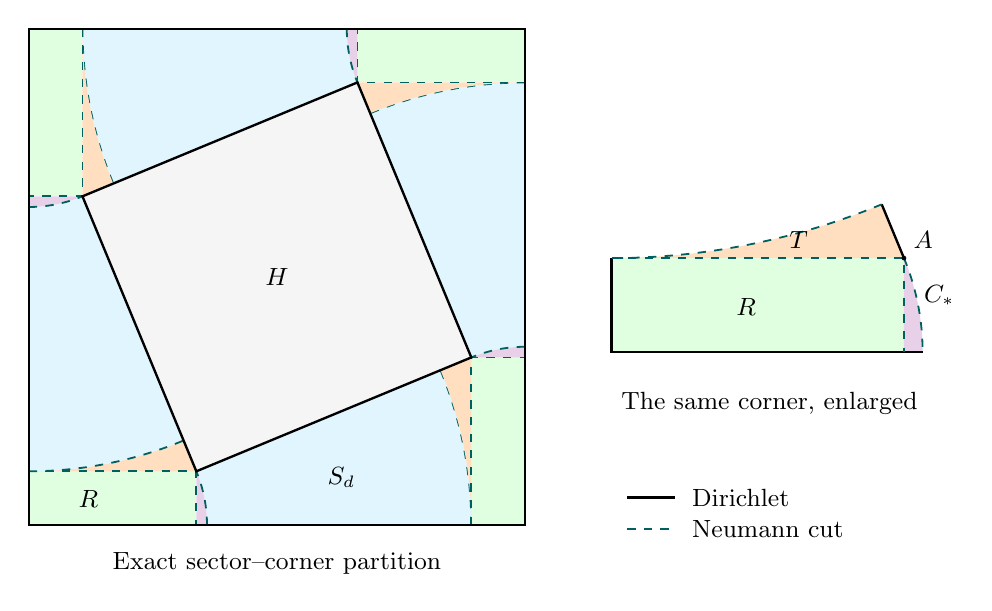
\begin{tikzpicture}[font=\small,
  physical/.style={draw=black,line width=.85pt},
  artificial/.style={draw=teal!75!black,dashed,line width=.65pt}]
 \pgfmathsetmacro{\ang}{22.5}
 \pgfmathsetmacro{\qc}{.6*cos(\ang)}
 \pgfmathsetmacro{\qs}{.6*sin(\ang)}
 \pgfmathsetmacro{\gap}{1-\qc-\qs}
 \pgfmathsetmacro{\dd}{\gap/2}
 \pgfmathsetmacro{\LL}{\dd+\qs}
 \pgfmathsetmacro{\BT}{\LL/tan(\ang)}
 \pgfmathsetmacro{\aa}{\dd/sin(\ang)}
 \pgfmathsetmacro{\bb}{\qc+\dd/tan(\ang)}
 \pgfmathsetmacro{\ox}{\LL-\dd/tan(\ang)}
 \pgfmathsetmacro{\ex}{\BT*sin(\ang)}
 \pgfmathsetmacro{\ey}{\dd+\BT*(1-cos(\ang))}
 \begin{scope}[scale=6.3]
  \foreach \turn in {0,90,180,270}{
   \begin{scope}[rotate around={\turn:(.5,.5)}]
    \path[fill=cyan!12] ({\ox+\aa},0)
      arc[start angle=0,end angle=\ang,radius=\aa]
      -- ({\ox+\bb*cos(\ang)},{\bb*sin(\ang)})
      arc[start angle=\ang,end angle=0,radius=\bb] -- cycle;
    \path[fill=green!12] (0,0) rectangle (\LL,\dd);
    \path[fill=orange!25] (0,\dd)--(\LL,\dd)--(\ex,\ey)
      arc[start angle={\ang-90},end angle=-90,radius=\BT]--cycle;
    \path[fill=violet!18] (\LL,0)--(\LL,\dd)
      arc[start angle=\ang,end angle=0,radius=\aa]--cycle;
    \draw[artificial] ({\ox+\aa},0)
      arc[start angle=0,end angle=\ang,radius=\aa];
    \draw[artificial] ({\ox+\bb},0)
      arc[start angle=0,end angle=\ang,radius=\bb];
    \draw[artificial] (0,\dd)--(\LL,\dd)--(\LL,0);
   \end{scope}
  }
  \path[fill=gray!8] (\LL,\dd)--({1-\dd},\LL)
       --({1-\LL},{1-\dd})--(\dd,{1-\LL})--cycle;
  \draw[physical] (0,0) rectangle (1,1);
  \draw[physical] (\LL,\dd)--({1-\dd},\LL)
       --({1-\LL},{1-\dd})--(\dd,{1-\LL})--cycle;
  \node at (.5,.5) {$H$};
  \node at (.63,.095) {$S_d$};
  \node at (.12,.052) {$R$};
  \node[anchor=north] at (.5,-.035) {Exact sector--corner partition};
 \end{scope}
 \begin{scope}[shift={(7.4cm,2.2cm)},scale=11]
  \path[fill=green!12] (0,0) rectangle (\LL,\dd);
  \path[fill=orange!25] (0,\dd)--(\LL,\dd)--(\ex,\ey)
       arc[start angle={\ang-90},end angle=-90,radius=\BT]--cycle;
  \path[fill=violet!18] (\LL,0)--(\LL,\dd)
       arc[start angle=\ang,end angle=0,radius=\aa]--cycle;
  \draw[physical] (0,\dd)--(0,0)--({\ox+\aa},0);
  \draw[physical] (\ex,\ey)--(\LL,\dd);
  \draw[artificial] (0,\dd)--(\LL,\dd)--(\LL,0);
  \draw[artificial] (\ex,\ey)
       arc[start angle={\ang-90},end angle=-90,radius=\BT];
  \draw[artificial] (\LL,\dd)
       arc[start angle=\ang,end angle=0,radius=\aa];
  \node at ({.46*\LL},{.48*\dd}) {$R$};
  \node at ({.64*\LL},{\dd+.021}) {$T$};
  \node[anchor=west] at ({\LL+.012},{.6*\dd}) {$C_*$};
  \node[circle,fill=black,inner sep=.6pt] at (\LL,\dd) {};
  \node[anchor=south west] at (\LL,\dd) {$A$};
  \node[anchor=north] at ({.54*\LL},-.035) {The same corner, enlarged};
 \end{scope}
 \draw[physical] (7.6cm,.35cm)--(8.2cm,.35cm);
 \node[anchor=west] at (8.3cm,.35cm) {Dirichlet};
 \draw[artificial] (7.6cm,-.05cm)--(8.2cm,-.05cm);
 \node[anchor=west] at (8.3cm,-.05cm) {Neumann cut};
\end{tikzpicture}
\caption{The exact partition, illustrated with
$q=3/5$, $\theta=\pi/8$, and equal bounding-box gaps.  These larger
gaps make the cap geometry visible; the estimates use the thin ranges
specified in the text.  Each cyan annular corridor has Dirichlet rays
and Neumann arcs.  Each corner is exactly the union of the rectangle
$R$, tangent cap $T$, and chord cap $C_*$; no area is discarded.}
\label{geo:partition-figure}
\end{figure}
\subsection{A radial Neumann count with its first root included}
\label{geo:radial}

We first establish the radial input, including its counting convention.
For $0<a<b$ and real $\nu\ge0$ consider
\[
 \mathcal L_\nu=-\frac{d^2}{dr^2}-\frac1r\frac d{dr}
                       +\frac{\nu^2}{r^2}
\]
in $L^2((a,b),r\,dr)$, with form domain $H^1(a,b)$ and form
$\int_a^b(r|u'|^2+\nu^2|u|^2/r)\,dr$.  Its operator conditions are
the ordinary radial conditions $u'(a)=u'(b)=0$.  The endpoints are
positive and regular; no condition at a Bessel singularity is involved.

Put
\[
 M_\nu(x)^2=J_\nu'(x)^2+Y_\nu'(x)^2,
 \qquad J_\nu'(x)+iY_\nu'(x)=M_\nu(x)e^{i\phi_\nu(x)},
\]
using the continuous phase with limit $\pi/2$ at zero.  The Wronskian
and Bessel equation give
\begin{equation}\label{geo:phase-derivative}
 \phi_\nu'(x)=\frac{2(x^2-\nu^2)}{\pi x^3M_\nu(x)^2}.
\end{equation}
We use the derivative-modulus inequality of Horsley
\cite[Theorem 2, equation (15), and Section 4, equation (58)]{Horsley2017}:
\begin{equation}\label{geo:horsley}
 \frac d{dx}\left(\frac{x^2M_\nu(x)^2}{\sqrt{x^2-\nu^2}}\right)<0,
 \qquad
 \frac{x^2M_\nu(x)^2}{\sqrt{x^2-\nu^2}}>\frac2\pi,
 \qquad x>\nu\ge0.
\end{equation}
The second inequality follows from the first and its limiting value
$2/\pi$ at infinity.  These are global inequalities for every real
nonnegative order, not asymptotic estimates with an unspecified onset.
Together with \eqref{geo:phase-derivative}, they imply
\begin{equation}\label{geo:phase-speed}
 \phi_\nu'(x)<\frac{\sqrt{x^2-\nu^2}}x\quad(x>\nu),
 \qquad \phi_\nu'(x)<0\quad(0<x<\nu).
\end{equation}
The phase derivative vanishes at the turning point when $\nu>0$.

For $\sigma>0$ define
\[
 F(\sigma)=\phi_\nu(b\sigma)-\phi_\nu(a\sigma),\qquad
 I_\nu(\sigma^2)=\frac1\pi\int_a^b
                       \sqrt{\sigma^2-\nu^2/r^2}_+\,dr.
\]
To identify the count, use the solution normalized at the left endpoint,
\begin{align*}
 u(r;\sigma)&=c_\sigma\bigl[
 Y_\nu'(a\sigma)J_\nu(r\sigma)
             -J_\nu'(a\sigma)Y_\nu(r\sigma)\bigr],
 &\hspace{35mm}c_\sigma=\frac{\pi a\sigma}{2}.
\end{align*}
The Wronskian $J_\nu Y_\nu'-J_\nu'Y_\nu=2/(\pi x)$ gives
$u(a;\sigma)=1$, $u_r(a;\sigma)=0$, and
\[
 u_r(b;\sigma)=-\sigma c_\sigma
       M_\nu(a\sigma)M_\nu(b\sigma)\sin F(\sigma).
\]
Thus a positive eigenvalue occurs precisely at an integer phase level.
At $F(\sigma)=j\pi$, the endpoint derivative vectors are proportional,
and the same Wronskian gives
\[
 b\,u(b;\sigma)\,\partial_\sigma u_r(b;\sigma)
       =-\frac2\pi c_\sigma^2M_\nu(a\sigma)^2F'(\sigma).
\]
Differentiating the radial equation in $\sigma$ gives the Lagrange identity
\[
 \frac d{dr}\left[r\bigl(u\,\partial_\sigma u_r
                  -u_r\,\partial_\sigma u\bigr)\right]
                 =-2\sigma r u^2.
\]
Its left endpoint term is zero.  At a Neumann root it therefore proves
\begin{equation}\label{geo:positive-crossing}
 F'(\sigma)=\frac{\pi\sigma}
  {c_\sigma^2M_\nu(a\sigma)^2}
                 \int_a^b r\,u(r;\sigma)^2\,dr>0.
\end{equation}
In particular, global monotonicity of $F$ is not being assumed.

If $\nu>0$, the small-argument expansions and
\eqref{geo:phase-derivative} show that
$-\pi/2<F(\sigma)<0$ for sufficiently small positive $\sigma$.
The large-argument expansions give
$F(\sigma)=(b-a)\sigma+o(1)$; the relevant standard function and
derivative expansions are recorded in \cite[Sections 10.7 and 10.17]{DLMF}.
Every integer-level crossing is upwards by
\eqref{geo:positive-crossing}.  There can be no negative integer-level
crossing, nor two crossings of the same integer level: either would
require an intervening contact with nonpositive derivative.  The first
eigenvalue is consequently the crossing $F=0$, followed by
$F=\pi,2\pi,\ldots$.  For $\nu=0$, the phase is increasing and
$F(\sigma)>0$ tends to zero as $\sigma\downarrow0$.  The positive roots
then start at $F=\pi$, and the constant function contributes the zero
eigenvalue.  Regular Sturm--Liouville uniqueness ensures that these
roots are precisely the simple radial eigenvalues.  We have thus proved,
including every positive energy endpoint,
\begin{equation}\label{geo:radial-floor}
 N_\nu^{NN}(\sigma^2)=1+
          \left\lfloor\frac{F(\sigma)}\pi\right\rfloor.
\end{equation}

Integrating \eqref{geo:phase-speed} from $a\sigma$ to $b\sigma$ yields
$F(\sigma)<\pi I_\nu(\sigma^2)$; strictness holds because the interval
has positive length and the derivative inequality is strict except
possibly at one point.  The forbidden part of the interval only helps.
Therefore
\begin{equation}\label{geo:radial-action}
 N_\nu^{NN}(E)<I_\nu(E)+1,
 \qquad N_\nu^{NN}(E)\le\lceil I_\nu(E)\rceil,
 \qquad E>0.
\end{equation}
In particular zero action gives zero count, even at a turning threshold.
At $E=0$ the counts are separately zero for $\nu>0$ and one for $\nu=0$.
This last distinction avoids applying the strict inequality at zero
energy to the constant Neumann mode.

\subsection{The scalar radial deficit}
\label{geo:scalar}

Write
\[
 R(y)=\sum_{m\ge1}\sqrt{y^2-m^2}_+,
 \qquad D(y)=\frac{\pi y}{4}-\frac{R(y)}y\quad(y>0),
 \qquad D(0)=0.
\]
We need only the following modest uniform lower bound:
\begin{equation}\label{geo:D-bound}
 D(y)\ge\frac7{20}\quad(y\ge1),
 \qquad D(y)=\frac{\pi y}{4}\quad(0\le y\le1).
\end{equation}
Here is a short analytic tail and a complete finite specification of the
small remaining interval.  For $y\ge1$, put $n=\lfloor y\rfloor$,
$h=y-n$, and $f(x)=\sqrt{y^2-x^2}$ on $[0,y]$.  Concavity on $[0,n]$
gives
\[
 \int_0^n f(x)\,dx\ge\frac y2+
              \sum_{m=1}^{n-1}f(m)+\frac{f(n)}2.
\]
Moreover,
\[
 \int_n^y f(x)\,dx
   =\int_0^h\sqrt{u(2y-u)}\,du
   \ge\frac23h^{3/2}\sqrt{2y-h}.
\]
It follows that
\[
 \frac{\pi y^2}{4}-R(y)
   \ge\frac y2-\sqrt{2y-h}\sqrt h\left(\frac12-\frac{2h}{3}\right).
\]
For $h\ge3/4$ the correction on the right is nonnegative.  For
$0\le h\le3/4$, the maximum of
$\sqrt h(1/2-2h/3)$ is $1/6$, attained at $h=1/4$.
Consequently
\begin{equation}\label{geo:D-tail}
 D(y)\ge\frac12-\frac1{\sqrt{18y}}>\frac7{20},
                       \qquad y\ge\frac52,
\end{equation}
where the last comparison is $1/45<9/400$.

For $1\le y\le5/2$, use the 75 closed intervals
$[a_j,b_j]=[1+j/50,1+(j+1)/50]$, $0\le j<75$.
The monotonicity of each radical gives the rigorous lower bound
\begin{equation}\label{geo:D-certificate}
 D(y)\ge\frac{333}{106}\frac{a_j}{4}
   -\sum_{m=1}^{\lfloor b_j\rfloor}
                   \sqrt{1-m^2/b_j^2},\qquad a_j\le y\le b_j.
\end{equation}
To evaluate it, for every nonnegative rational $x$ let
\[
 n_x=\left\lfloor\sqrt{\left\lfloor2^{100}x\right\rfloor}\right\rfloor,
 \qquad \sqrt{x}<\frac{n_x+1}{2^{50}}.
\]
Integer squaring verifies both this strict upper bound and
$(n_x/2^{50})^2\le x$.  The inequality $333/106<\pi$ is checked using
$\pi=16\arctan(1/5)-4\arctan(1/239)$ and the first twelve terms of each
alternating series, with its next term as remainder bound.  Substituting
the radical upper bounds in \eqref{geo:D-certificate}, exact rational
arithmetic gives a lower bound at least
\[
 \frac{36535721}{100000000}>\frac7{20}
\]
on every interval.  The supplied verifier
\texttt{verify\_radial\_scalar.py} performs exactly these 75 tests,
checks the adjoining endpoints, and uses integer and rational arithmetic
only.  Its explicit failure checks are unaffected by Python's
\texttt{-O} option.  Equations \eqref{geo:D-tail} and
\eqref{geo:D-certificate} prove \eqref{geo:D-bound} for all real $y$.

An averaging consequence will be important at small inner radii.  If
$0\le u<v$ and $v\ge1$, then
\begin{equation}\label{geo:D-average}
 \int_u^vD(y)\,dy\ge\frac7{20}(v-u).
\end{equation}
If $u\ge1$ this is pointwise.  Otherwise the average on $[u,1]$ is
$\pi(1+u)/8\ge\pi/8>7/20$, and the remaining interval is covered by
\eqref{geo:D-bound}.

\subsection{The true-area corridor saving}
\label{geo:corridor-count}

On a sector with Dirichlet rays and Neumann arcs the angular orders are
$\nu_m=m\pi/\theta$, $m\ge1$.  By \eqref{geo:radial-action}, its count
is bounded by the sum of the ceilings of
\[
 I_m=\int_a^b\sqrt{t^2-m^2/(\theta\rho)^2}_+\,d\rho.
\]
The channels with $m\ge\theta bt$ have zero action and zero count;
including equality in $M=\lfloor\theta bt\rfloor$ is harmless.  Thus
\begin{align}
 N_{S_z}(\pi^2t^2)
 &\le\sum_{m=1}^{M}\lceil I_m\rceil\notag\\
 &\le\frac{\pi}{4}|S_z|t^2
       -t\int_{a(z)}^{b(z)}D(\theta\rho t)\,d\rho
       +\lfloor\theta b(z)t\rfloor.\label{geo:sector-count}
\end{align}
This has the true sector area coefficient.  If $\theta b(z)t<1$, the
count is zero.  Otherwise \eqref{geo:D-average} shows that the normalized
Weyl saving is at least
$\tfrac7{20}\mathcal L(z)-\theta b(z)$.

Define the two budgets
\begin{align}
 \mathcal A(z)&=\frac7{20}\mathcal L(z)-\theta b(z),\notag\\
 \mathcal B(z)&=\frac\pi4|S_z|t
        =\frac{\pi\theta t}{8}
                    (c^2+2cz\cot\theta-z^2),\notag\\
 \mathcal G(z)&=\min\{\mathcal A(z),\mathcal B(z)\}.
                                                    \label{geo:budgets}
\end{align}
The first budget applies to an active sector; the second is its exact
saving if inactive.  Hence $t\mathcal G(z)$ is always a valid saving.
The identity
\[
 \theta b(g)=\theta\cot\theta\,w\le w
\]
and \eqref{geo:coarse-geometry} show that
$\mathcal A(z)\ge2337/10000>0$; $\mathcal B$ is nonnegative as well.
The function $\mathcal A$ is affine, and $\mathcal B$ is concave, so
$\mathcal G$ is concave: its hypograph is the intersection of their
convex hypographs.  Consequently
\[
 \mathcal G(z)+\mathcal G(g-z)\ge\mathcal G(0)+\mathcal G(g).
\]
The two opposite-gap identities therefore give the uniform placement
bound
\begin{equation}\label{geo:sector-total}
 \sum_{z\in\{\ell,r,d,h\}}N_{S_z}(\pi^2t^2)
 \le\frac\pi4\left(\sum_z|S_z|\right)t^2
                  -2t\bigl(\mathcal G(0)+\mathcal G(g)\bigr).
\end{equation}
Also $\mathcal B$ increases on $[0,g]$, because its derivative has the
sign of $c\cot\theta-z>0$ by \eqref{geo:coarse-geometry}.

\subsection{An elementary action estimate for decreasing potentials}
\label{geo:action-log}

The cap models require a different one-dimensional estimate.  Let $V$
be nonnegative, smooth and strictly decreasing on $(0,L)$, with
$V(0+)=+\infty$, and use the Friedrichs Dirichlet form
\[
 \int_0^L(|u'|^2+V|u|^2),\qquad
 \{u\in H^1_0(0,L):\int_0^LV|u|^2<\infty\}.
\]
For every $E>0$ its inclusive count satisfies
\begin{equation}\label{geo:action-log-bound}
 N_V(E)\le\frac1\pi\int_0^L\sqrt{E-V}_+\,dx+\mathcal H(L\sqrt E),
 \qquad
 \mathcal H(z)=\frac12+\frac1{2\pi}\log_+z.
\end{equation}
To see this, put $p=\sqrt{E-V}_+$.  If $p(L)\le1/L$, then
$V\ge E-L^{-2}$, and the DD kinetic lower bound $\pi^2/L^2$ makes
the inclusive count zero.  Otherwise let $x_0$ be the unique point
where $p(x_0)=1/L$ and introduce a Neumann cut there.  On $(0,x_0)$,
the first eigenvalue is at least
\[
 E-L^{-2}+\frac{\pi^2}{4x_0^2}>E,
\]
so this piece contributes no count.  This comparison remains valid for
the singular left endpoint because its Friedrichs form has zero trace.
On the right interval solve $u(x_0)=1$, $u'(x_0)=0$ and define
\[
 u=\rho\sin\vartheta,\quad u'=p\rho\cos\vartheta,
 \quad\vartheta(x_0)=\pi/2.
\]
Differentiation gives
\[
 \vartheta'=p+\frac{p'}{2p}\sin(2\vartheta)
                     \le p+\frac{p'}{2p}.
\]
At a zero of $u$, the phase crosses an integer multiple of $\pi$
upwards, with derivative $p>0$.  Sturm oscillation for the N--D
interval gives the inclusive count $\lfloor\vartheta(L)/\pi\rfloor$;
an endpoint zero is counted.  Integration bounds it by
\[
 \frac12+\frac1\pi\int_{x_0}^Lp\,dx
                   +\frac1{2\pi}\log(Lp(L)),
\]
which proves \eqref{geo:action-log-bound}.

\subsection{The tangent cap and its Kelvin endpoint}
\label{geo:kelvin}

Translate the top contact to zero and invert by
\[
 (u,v)=\frac{(x,y)}{x^2+y^2}.
\]
The tangent line and circle become the Neumann lines $v=0$ and
$v=h_0=1/(2B_T)$.  The Dirichlet hole edge
$x\cos\theta+y\sin\theta=B_T\sin\theta$ becomes $u=U(v)$, where
\[
 U(v)=h_0\cot\theta+
        \sqrt{h_0^2\csc^2\theta-(v-h_0)^2},\qquad0<v<h_0.
\]
The image is $u>U(v)$, and $\min U=U(0)=\cot\theta/B_T=:U_0$.
Zero extension into the product strip
$u>U_0$, $0<v<h_0$ crosses only this Dirichlet crosscut; it does not
move a Neumann boundary.  Dirichlet energy is invariant under this
two-dimensional conformal or anticonformal map.  Its exact mass is
\[
 \int |F(u,v)|^2(u^2+v^2)^{-2}\,du\,dv.
\]
Replacing the weight by the larger $u^{-4}$ lowers all Rayleigh
quotients.  The two weights are comparable on the strip because
$v/u\le h_0/U_0$, so the extension maps into the finite-mass model
form domain.  Its count is consequently an upper bound for the cap count.
More explicitly, the model form domain is
\[
 \mathcal V=\left\{F\in H^1_{\rm loc}((U_0,\infty)\times(0,h_0)):
 F|_{u=U_0}=0,\quad
 \int\bigl(|\nabla F|^2+u^{-4}|F|^2\bigr)\,du\,dv<\infty\right\}.
\]
There is no boundary restriction at infinity or on the two horizontal
sides.  The Neumann cosine expansion in the transverse variable is an
orthogonal decomposition of both its energy and weighted mass.

Separate the transverse NN modes $\mu_m=m\pi/h_0$, $m\ge0$.
For $x=1/u$ and $F(u)=G(x)/x$ one has $0<x<L=1/U_0=B_T\tan\theta$,
and direct substitution gives
\begin{align*}
 \int_{U_0}^{\infty}u^{-4}|F|^2\,du&=\int_0^L|G|^2\,dx,\\
 \int_{U_0}^{\infty}|F'|^2\,du
       &=\int_0^L|G'|^2\,dx-\left[\frac{|G|^2}{x}\right]_0^L,\\
 \mu_m^2\int_{U_0}^{\infty}|F|^2\,du
       &=\int_0^L\mu_m^2x^{-4}|G|^2\,dx.
\end{align*}
The resulting operator is exactly the Friedrichs DD realization of
\begin{equation}\label{geo:kelvin-operator}
 -G''+\mu_m^2x^{-4}G.
\end{equation}
Here the endpoint at infinity deserves attention.  For the zero mode,
$F(U_0)=0$ and $F'\in L^2(U_0,\infty)$ imply $F(u)=o(\sqrt u)$:
split the derivative integral at a fixed large point and apply
Cauchy--Schwarz to its tail.  Hence $G(x)^2/x\to0$ at zero, and
$G(0)=0$.  The half-line Hardy inequality gives
$\int_{U_0}^{\infty}|F|^2/u^2\le4\int_{U_0}^{\infty}|F'|^2$,
and $G'(x)=F(1/x)-x^{-1}F'(1/x)$ then gives $G'\in L^2(0,L)$.
Conversely, closing the compactly supported identity above gives the
whole DD form.  Cutoffs at strip infinity are dense in the original
natural form: truncate the function values first, then let the cutoff
interval length tend to infinity.  Its added energy tends to zero.
Thus a finite-energy constant limit of $F$ is allowed and corresponds
to $G$ proportional to $x$; no extra physical Dirichlet condition has
been imposed at the cusp.

The zero channel of \eqref{geo:kelvin-operator} has count
$\lfloor Lt\rfloor\le Lt$.  A positive channel can contribute only if
$m\le h_0L^2t$.  Apply \eqref{geo:action-log-bound} to those channels,
and bound the decreasing sum of their actions by the integral over
all nonnegative real orders.  This gives
\[
 \sum_{m\ge1}\int_0^L
       \sqrt{t^2-\frac{m^2}{h_0^2x^4}}_+\,dx
       \le\frac{\pi t^2}{4}\int_0^Lh_0x^2\,dx.
\]
With $W=h_0L^2=L\tan\theta/2$ and
$A_T^{\rm mod}=h_0L^3/3=B_T^2\tan^3\theta/6$, we conclude
\begin{equation}\label{geo:top-count}
 N_T(\pi^2t^2)\le\frac\pi4A_T^{\rm mod}t^2
                  +Lt+\lfloor Wt\rfloor\mathcal H(\pi Lt).
\end{equation}
Its leading area excess is not discarded.  Writing $z=\tan\theta$,
\begin{equation}\label{geo:top-area-error}
 A_T^{\rm mod}-|T|
  =\frac{B_T^2}{2}\left(\frac{z^3}{3}-z+\arctan z\right)
  =\frac{B_T^2}{2}\int_0^z\frac{v^4}{1+v^2}\,dv
  \le\frac{L^2\tan^3\theta}{10}.
\end{equation}

\subsection{The chord cap and its zero angular channel}
\label{geo:mobius}

Place the right-cap circle center at zero, and put
$A_+=a\cos\theta+id$, $A_-=a\cos\theta-id$.  The M\"obius map
\[
 z=-\frac{\zeta-A_+}{\zeta-A_-}
\]
takes the upper circular segment exactly onto
$0<|z|<1$, $0<\arg z<\theta$.  On the chord it equals
$(d-y)/(d+y)>0$, the circular arc has argument $\theta$, and the
bottom real segment has modulus one.  Thus the two rays are Neumann
and the outer arc is Dirichlet.  Its pole is outside the half cap, and
the map is nondegenerate at the vertex sent to zero.  The inverse
derivative has squared modulus $4d^2/|1+z|^4$.

For $z=\rho e^{i\varphi}$,
\[
 |1+z|^2=(1+\rho)^2-4\rho\sin^2(\varphi/2)
              \ge(1+\rho)^2\cos^2(\theta/2).
\]
Set $\gamma=\sec^4(\theta/2)$ and $t'=\sqrt\gamma\,t$.
The actual cap count at $E$ is at most the count at $\gamma E$ of the
radial mass model $4d^2/(1+\rho)^4$ on the same wedge.  This is a mass
comparison on a fixed form domain, not Neumann domain monotonicity.
The substitution
\[
 x=\frac{2d\rho}{1+\rho},\quad0<x<d,\qquad
 f(x)=x\left(1-\frac{x}{2d}\right)
\]
transforms the metric to $dx^2+f(x)^2d\varphi^2$.  Its model area is
\[
 A_C^{\rm mod}=\theta\int_0^df(x)\,dx=\frac{\theta d^2}{3}.
\]
For angular NN order $\nu_m=m\pi/\theta$, $m\ge0$, the form and mass are
\begin{equation}\label{geo:weighted-cap-form}
 \int_0^d\left(f|u'|^2+\frac{\nu_m^2}{f}|u|^2\right)dx,
 \qquad \int_0^df|u|^2dx.
\end{equation}
The form domain has trace $u(d)=0$ and finite displayed energy at zero.
This is the regular sector condition; for $m=0$ it allows a nonzero
constant limit, whereas the logarithmic solution has infinite energy.

For $m\ge1$, $G=\sqrt f\,u$ gives the Friedrichs DD operator
\[
 -G''+\frac{\nu_m^2-1/4}{f^2}G,
 \qquad 2ff''-(f')^2=-1.
\]
The transformation is first an identity on compactly supported forms
and then by closure.  For eigenfunctions the regular behavior
$u=O(x^{\nu_m})$ also makes its endpoint term vanish.
Put $\beta=\sqrt{1-\theta^2/(4\pi^2)}$.  Since
$\nu_m^2-1/4\ge\beta^2\nu_m^2$, replacing the potential by
$\beta^2\nu_m^2/f^2$ lowers the eigenvalues.  This nonnegative potential
is strictly decreasing on $(0,d)$, so \eqref{geo:action-log-bound}
applies at energy $\pi^2t'^2$.

The number of channel errors is determined before this replacement.
The original form \eqref{geo:weighted-cap-form} gives
$\lambda\ge\nu_m^2/\max f^2=4\nu_m^2/d^2$, so only
$m\le\theta dt'/2$ can contribute.  It is safe to enlarge the
nonnegative action sum to all $m\ge1$ while keeping this original
cutoff for the error terms.  The decreasing-sum integral then bounds
the action sum by $\pi A_C^{\rm mod}t'^2/(4\beta)$.

For $m=0$ the critical negative potential must not be dropped.  Instead
let $-(fu')'=\lambda fu$, $\lambda>0$, and set
$v=fu'$, $G=v/\sqrt f=\sqrt f\,u'$.  Direct differentiation gives
\begin{equation}\label{geo:partner}
 -G''+V_+(x)G=\lambda G,
 \qquad
 V_+=\frac{3(f')^2}{4f^2}-\frac{f''}{2f}>0.
\end{equation}
A regular original eigenfunction satisfies
$u(x)=C-\lambda Cx^2/4+O(x^3)$, and hence
$G(x)=-\lambda Cx^{3/2}/2+O(x^{5/2})$.
The partner potential is $3/(4x^2)+O(1/x)$; its other local solution
has exponent $-1/2$ and is not square integrable.  Thus zero is the
limit-point, Dirichlet-trace endpoint of the partner.  At $d$,
$v'(d)=-\lambda f(d)u(d)=0$ and $f'(d)=0$, so $G'(d)=0$.
Conversely, any positive partner eigenfunction gives
\[
 u=-\frac{(\sqrt f\,G)'}{\lambda f},\qquad u'=\frac G{\sqrt f},
\]
which is regular at zero and vanishes at $d$.  These transformations
are inverse on positive eigenspaces.  The original has no zero mode
because zero energy forces a constant with $u(d)=0$; the partner has
none because its form is positive.  There is therefore no deleted
ground state or exceptional lost eigenvalue.

Since $V_+\le C_d/x^2$, Hardy's inequality shows that the partner form
domain is $\{G\in H^1(0,d):G(0)=0\}$.  Its form dominates the ordinary
D--N kinetic form, whose eigenvalues are $((j-1/2)\pi/d)^2$, $j\ge1$.
Consequently its inclusive count, and the original zero-channel count,
are at most $\lfloor dt'+1/2\rfloor$.  Combining all channels gives
\begin{equation}\label{geo:right-count}
 N_{C_*}(\pi^2t^2)\le\frac\pi4\frac{\gamma A_C^{\rm mod}}\beta t^2
      +\lfloor dt'+1/2\rfloor
      +\left\lfloor\frac{\theta dt'}2\right\rfloor
                                        \mathcal H(\pi dt').
\end{equation}
Finally, sine concavity on $[0,\theta]$ gives
\[
 |C_*|=a^2\int_0^\theta\sin^2\varphi\,d\varphi
       \ge\frac{a^2\sin^2\theta\,\theta}{3}
       =A_C^{\rm mod}.
\]
The full excess over the true area, including the energy and angular
comparisons, is therefore bounded by
\begin{equation}\label{geo:right-area-error}
 \frac{\gamma A_C^{\rm mod}}\beta-|C_*|
       \le\frac{\theta d^2}{3}\left(\frac\gamma\beta-1\right).
\end{equation}


\begin{figure}[tb]
\centering
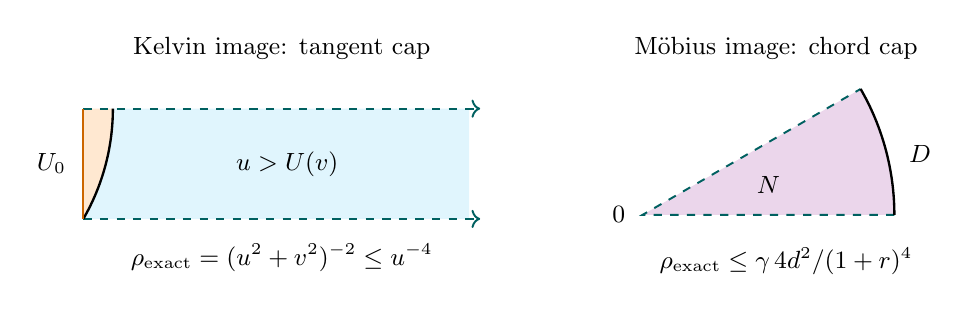
\begin{tikzpicture}[font=\small,
  dside/.style={draw=black,line width=.85pt},
  nside/.style={draw=teal!75!black,dashed,line width=.7pt}]
 \begin{scope}[scale=1.4]
  \path[fill=cyan!12] (0,0)
     plot[domain=0:1,samples=35] ({sqrt(4-(\x-1)^2)-sqrt(3)},\x)
     --(3.5,1)--(3.5,0)--cycle;
  \path[fill=orange!18] (0,0)
     plot[domain=0:1,samples=35] ({sqrt(4-(\x-1)^2)-sqrt(3)},\x)
     --(0,1)--cycle;
  \draw[nside,->] (0,0)--(3.6,0);
  \draw[nside,->] (0,1)--(3.6,1);
  \draw[dside] plot[domain=0:1,samples=35]
                   ({sqrt(4-(\x-1)^2)-sqrt(3)},\x);
  \draw[orange!80!black,line width=.7pt] (0,0)--(0,1);
  \node[anchor=east] at (-.07,.5) {$U_0$};
  \node at (1.85,.5) {$u>U(v)$};
   \node[anchor=south] at (1.8,1.36) {Kelvin image: tangent cap};
  \node[anchor=north] at (1.8,-.14)
       {$\rho_{\rm exact}=(u^2+v^2)^{-2}\le u^{-4}$};
 \end{scope}
 \begin{scope}[shift={(7.1cm,.05cm)},scale=3.2]
  \path[fill=violet!16] (0,0)--(1,0)
       arc[start angle=0,end angle=30,radius=1]--cycle;
  \draw[nside] (1,0)--(0,0)--({cos(30)},{sin(30)});
  \draw[dside] (1,0) arc[start angle=0,end angle=30,radius=1];
  \node[anchor=east] at (-.03,0) {$0$};
  \node at (.5,.12) {$N$};
  \node[anchor=west] at (1.02,.24) {$D$};
  \node[anchor=south] at (.53,.58) {M\"obius image: chord cap};
  \node[anchor=north] at (.57,-.09)
       {$\rho_{\rm exact}\le\gamma\,4d^2/(1+r)^4$};
 \end{scope}
\end{tikzpicture}
\caption{The two conformal comparison domains.  On the left the thin
orange region is added by zero extension across the Dirichlet curve
$u=U(v)$ to the Dirichlet line $u=U_0$; the horizontal sides remain
Neumann and continue to infinity.  On the right the chord and circle
become Neumann rays, while the physical Dirichlet side becomes $r=1$.
For visibility the displayed angle is $\pi/6$; the left coordinates are
$(u/h_0-2\cot\theta,v/h_0)$, and the right radius is unchanged.
Only the written mass inequalities, not the drawn areas, are used in
the comparison.}
\label{geo:cap-maps}
\end{figure}
\subsection{Rectangle counts and two forms of the corner bound}
\label{geo:combined-corners}

The mixed rectangle eigenvalues are
$\pi^2((j+1/2)^2/L^2+(k+1/2)^2/d^2)$, $j,k\ge0$.
Write $A_1(y)=\sum_{j\ge0}\sqrt{y^2-(j+1/2)^2}_+$.
The scalar midpoint bound \eqref{eq:rect-midpoint} is
$A_1(y)\le\pi y^2/4+4y/25$.
Summing one index and using $\lfloor v+1/2\rfloor\le v+1/2$ gives
\begin{equation}\label{geo:rectangle-constant}
 N_R(\pi^2t^2)\le\frac\pi4Ldt^2
                      +\left(\frac4{25}d+\frac L2\right)t+\frac14.
\end{equation}
Indeed the radical sum is $(d/L)A_1(Lt)$, and the remaining half-count
is at most $\tfrac12\lfloor Lt+1/2\rfloor\le Lt/2+1/4$.
Interchanging $L,d$ gives the other version.  Averaging yields excess
at most $33(L+d)t/100+1/4$.  If the rectangle is active, its first
eigenvalue implies $(L+d)t\ge\sqrt2$.  If inactive, its count is zero.
Thus at every energy we also have
\begin{equation}\label{geo:rectangle-absorbed}
 N_R(\pi^2t^2)\le\frac\pi4Ldt^2+\frac{51}{100}(L+d)t,
\end{equation}
since $33/100+1/(4\sqrt2)<51/100$.

Let $\Delta$ denote the sum of the model-area excesses of the eight caps.
Equations \eqref{geo:corner-sums}, \eqref{geo:top-area-error}, and
\eqref{geo:right-area-error} give
\begin{equation}\label{geo:area-excess}
 \Delta\le\frac25w^2\tan^3\theta
        +\frac23\theta g^2\left(\frac\gamma\beta-1\right).
\end{equation}
If $\gamma/\beta-1\le3\theta^2/5$, this is at most
$\tfrac25(w^2\tan^3\theta+\theta^3g^2)$.
The sum of the positive-channel multiplicities, divided by $t$, is at
most
\begin{equation}\label{geo:channel-total}
 2w\tan\theta+\theta g\sqrt\gamma.
\end{equation}
If $\mathcal H_*$ bounds all the cap logarithmic factors, retaining the
constants in \eqref{geo:rectangle-constant} gives the following total
corner excess over the true area term:
\begin{align}
 &\sum_{\rm corners}N(\pi^2t^2)
                   -\frac\pi4|\text{all corners}|t^2\notag\\
 &\quad\le\frac\pi4\Delta t^2
   +t\left[\left(\frac{83}{25}+2\sqrt\gamma\right)g
                                      +\frac{116}{25}s\right]+3
   +t(2w\tan\theta+\theta g\sqrt\gamma)\mathcal H_*.
                                                    \label{geo:corner-budget}
\end{align}
The constant three is four rectangle quarters plus four right-cap
halves.  For the very thin range it is preferable instead to use
\eqref{geo:rectangle-absorbed} and
$\lfloor v+1/2\rfloor\le2v$, valid for every $v\ge0$.

\subsection{Closing the all-energy thin range}
\label{geo:thin-all}

Assume $0<\delta\le1/50$.  Elementary Taylor bounds and feasibility give
\begin{equation}\label{geo:very-thin-geometry}
 \theta<\frac1{40},\quad\theta\le\frac{21}{20}\delta,
 \quad\tan\theta\le\frac{53}{50}\delta,
 \quad w\le\frac{51}{50}\delta,
 \quad c,\mathcal L(z)\ge\frac{97}{100},
 \quad\theta\cot\theta\ge\frac{99}{100}.
\end{equation}
For example $\cos(1/40)+\sin(1/40)>50/49$, and on this smaller interval
$\cos\theta+\sin\theta-1\ge(987/1000)\theta$.
The remaining estimates follow from
$\tan\theta\le\theta/(1-\theta^2/2)$,
$w\le\delta+\theta^2/2$, and \eqref{geo:sector-geometry}.
Also
\begin{equation}\label{geo:gamma-small}
 \sqrt\gamma\le\frac{1001}{1000},\qquad
 \frac\gamma\beta-1\le\frac35\theta^2.
\end{equation}
More generally the second bound holds for $z=\theta^2\le1/100$:
\[
 \gamma\le(1-z/4)^{-2}\le1+\frac{51}{100}z,
 \qquad
 \beta^{-1}\le(1-z/36)^{-1/2}\le1+\frac3{200}z.
\]
Squaring and clearing positive denominators proves these scalar
inequalities on that interval, and their product is at most $1+3z/5$.
The stronger first bound in \eqref{geo:gamma-small} uses
$\theta<1/40$.

Using the absorbed rectangle bound and the bound $2dt'$ for the right
zero channel, the linear corner cost is less than
$(1017/100)\delta t$.  Indeed it is at most
$(51/100)4wt+4wt+4g\sqrt\gamma\,t$.
Furthermore \eqref{geo:area-excess} and \eqref{geo:channel-total} give
\[
 \Delta<\frac{24}{25}\delta^5,
 \qquad 2w\tan\theta+\theta g\sqrt\gamma
                                      <\frac{161}{50}\delta^2.
\]
The first rational comparison is
\[
 \frac25\left(\frac{51}{50}\right)^2
             \left(\frac{53}{50}\right)^3
       +\frac25\left(\frac{21}{20}\right)^3<\frac{24}{25}.
\]
For $t\le216\delta^{-3}$ every logarithm argument is below
$700\delta^{-2}$.  The normalized total corner excess is consequently
bounded by
\begin{equation}\label{geo:thin-error}
 F_0(\delta)=\frac{1017}{100}\delta+163\delta^2
  +\frac{161}{50}\delta^2
                 \left(\frac12+\frac16\log(700\delta^{-2})\right).
\end{equation}
Each term increases on $(0,1/50]$.  Since
$\log(1750000)<15$ (for instance $e^3>20$ gives
$e^{15}>20^5>1750000$),
\[
 F_0(\delta)\le\frac{2034}{10000}+\frac{163}{2500}
                        +\frac{483}{125000}
                   =0.272464<\frac7{25}.
\]

For the sectors, \eqref{geo:very-thin-geometry} gives
$\mathcal A(z)\ge31/100$.  Directly from \eqref{geo:budgets},
\begin{align*}
 \mathcal B(0)+\mathcal B(g)
  &=\frac{\pi t}{4}
       \left[\theta\left(c^2-\frac{g^2}{2}\right)
                                      +cg\,\theta\cot\theta\right]\\
  &\ge\frac{47\pi}{200}t(\theta+g)
   \ge\frac{47\pi}{200}X.
\end{align*}
Both bracket coefficients are at least $47/50$, and
$\theta+g\ge\delta$ follows from
$\cos\theta+\sin\theta-1\le\theta$.  The inequality
$\min(a,x)+\min(a,y)\ge\min(a,x+y)$ now shows that the normalized
sector saving is at least
\[
 2\min\left\{\frac{31}{100},\frac{47\pi}{200}X\right\}
                         >\frac7{20}\qquad(X\ge1/4).
\]
This pays the entire corner excess \eqref{geo:thin-error}, so
\eqref{geo:target} holds for
$1/(4\delta)\le t\le216\delta^{-3}$.

For the low-energy endpoint, the common-core comparison
\eqref{rot:core-first} gives
\begin{equation}\label{geo:core-zero}
 N_{Q\setminus H}(\pi^2t^2)=0\qquad(X<1/\sqrt2).
\end{equation}
In particular this covers $X<1/4$.  Finally the arithmetic subtraction
tail \eqref{arith:subtraction-tail} applies for
$t\ge(5832/125)\delta^{-3}$, hence certainly for
$t\ge216\delta^{-3}$.  The ranges overlap and include their joining
endpoints.  At $E=0$ the original Dirichlet count is zero.  This completes
the all-energy assertion for $q\ge49/50$ at positive angle.

\subsection{Closing the remaining high-energy range}
\label{geo:high-energy-bridge}

We now assume $0<\delta\le2/25$ and $X\ge8$.  Set
$K=5832/125$.  By \eqref{arith:subtraction-tail}, only the window
\begin{equation}\label{geo:bridge-window}
 \frac8\delta\le t\le K\delta^{-3}
\end{equation}
remains.  The geometry \eqref{geo:coarse-geometry} and the same polynomial
bounds used above give
\[
 \sqrt\gamma\le\frac{1003}{1000},\qquad
 \frac\gamma\beta-1\le\frac35\theta^2.
\]
Every logarithm argument in the cap bounds is at most
$\pi\max(w,g\sqrt\gamma)t<160\delta^{-2}$.  Thus we may put
\[
 H_\delta=\frac12+\frac16\log(160\delta^{-2}).
\]
The product $\delta^2H_\delta$ is increasing on $(0,2/25]$, since its
derivative is
$\delta[2/3+\log(160\delta^{-2})/3]>0$.
At the right endpoint, $\log(25000)<11$, and hence
\begin{equation}\label{geo:bridge-log}
 \delta^2H_\delta<\frac4{625}\frac73.
\end{equation}
For example $e^3>20$ and $e^2>7$, from finite positive Taylor sums,
give $e^{11}>56000$.  We bound the product in
\eqref{geo:bridge-log}, not $H_\delta$ alone as $\delta\downarrow0$.

First take $\theta\ge\delta/10$.  We already have
$\mathcal A(z)\ge2337/10000$.  Moreover
\[
 \mathcal B(g)\ge\mathcal B(0)
     =\frac{\pi\theta t c^2}{8}
     \ge\frac\pi{10}\left(\frac{91}{100}\right)^2
     >\frac{24843}{100000}.
\]
Here the energy hypothesis is exactly $X\ge8$.  The four-sector saving
in \eqref{geo:sector-total}, divided by $t$, is at least $2337/2500$.
For the corners, \eqref{geo:corner-budget} gives linear coefficient at
most $(2663/500)w\le(141139/25000)\delta$.  The elementary comparisons
\[
 \frac25\left[\left(\frac{53}{50}\right)^2
                         \left(\frac65\right)^3
                        +\left(\frac76\right)^3\right]<\frac{71}{50},
 \qquad
 2\frac{53}{50}\frac65+\frac76\frac{1003}{1000}<\frac{93}{25}
\]
bound the area and positive-channel coefficients.  Since $\pi K/4<36.66$,
the area contribution divided by $t$ is at most $(521/10)\delta^2$.
Also $3/t\le3\delta/8$.  The total normalized corner error is thus at most
\[
 \frac{141139}{25000}\delta+\frac{521}{10}\delta^2
                 +\frac{93}{25}\delta^2H_\delta+\frac{3\delta}{8}.
\]
It increases in $\delta$ and, by \eqref{geo:bridge-log}, is at most
\[
 0.4516448+0.33344+0.055552+0.03
     =\frac{136037}{156250}=0.8706368<\frac{2337}{2500}.
\]
The exact residual margin is $20051/312500>1/50$.

For $\theta\le\delta/10$, use instead
\begin{equation}\label{geo:small-angle-geometry}
 \tan\theta\le\frac{1001}{10000}\delta,\quad
 w\le\frac{1001}{1000}\delta,\quad
 \mathcal L(z)\ge\frac{919}{1000},\quad
 \sqrt\gamma\le\frac{1001}{1000},\quad g\ge\frac9{10}\delta.
\end{equation}
These follow from $\theta\le1/125$,
$w\le\delta+\delta^2/200$, and
\[
 \mathcal L(z)\ge q-\frac{\delta^2}{200}
                         -\frac{1001}{20000}\delta^2>\frac{919}{1000}.
\]
The last inequality in \eqref{geo:small-angle-geometry} is
$g\ge\delta-\theta$.  At the maximal-gap endpoint,
\[
 \mathcal A(g)\ge\frac7{20}\frac{919}{1000}
                   -\frac{1001}{1000}\frac2{25}
               =\frac{24157}{100000}.
\]
As $b(g)>a(g)$ and $\theta a(g)\ge g$,
\[
 \mathcal B(g)\ge\frac\pi4\mathcal L(g)gt
     \ge\frac34\frac{919}{1000}\frac9{10}X\ge4.9626.
\]
Hence $\mathcal G(g)\ge24157/100000$, while $\mathcal G(0)\ge0$.
The normalized four-sector saving is at least $24157/50000=0.48314$.

The corresponding linear corner coefficient is at most
$(2661/500)(1001/1000)\delta=5.327322\delta$.  The area and channel
bounds become
\[
 \Delta\le\frac25\left[
        \left(\frac{1001}{1000}\right)^2
        \left(\frac{1001}{10000}\right)^3+\frac1{1000}\right]\delta^5
             <\frac{803}{1000000}\delta^5,
\]
and
\[
 2w\tan\theta+\theta g\sqrt\gamma
 \le\left[2\frac{1001}{1000}\frac{1001}{10000}
                          +\frac1{10}\frac{1001}{1000}\right]\delta^2
                   <\frac{301}{1000}\delta^2.
\]
In \eqref{geo:bridge-window}, the area term divided by $t$ is less than
$3\delta^2/100$.  The normalized corner error is consequently below
\[
 5.327322\delta+\frac3{100}\delta^2
                    +\frac{301}{1000}\delta^2H_\delta+\frac{3\delta}{8}.
\]
All terms increase in $\delta$.  Its endpoint bound is
\[
 \frac{8641363}{18750000}=0.460872693333\ldots
                         <\frac{24157}{50000},
\]
leaving the exact margin $52189/2343750>1/50$.

The two angle ranges overlap at $\theta=\delta/10$ and exhaust all
positive feasible rotations.  In both ranges, summing the exact piece
areas and their bounds proves \eqref{geo:target}; in fact the relaxed
mixed count is at most its Weyl term minus $t/50$ throughout
\eqref{geo:bridge-window}.  The arithmetic tail covers every larger
$t$, including the shared endpoint.  We have proved the desired
high-energy comparison for every $q\ge23/25$ and $X\ge8$.

Together with the all-energy result for $q\ge49/50$, the remaining
bounded slab in this size range is
\[
 \frac{23}{25}\le q\le\frac{49}{50},\qquad
 \frac14\le X\le8,\qquad t\le400.
\]
The low-energy zero range follows directly from \eqref{geo:core-zero}.
The analytic comparison includes $X=8$, so it joins the closed finite
certificate for this slab without an endpoint gap.

% Arithmetic fragment.  No theorem-like environments or local macros.
% The labels app:circle and arith:subtraction-tail are shared interfaces.
\section{An explicit circle estimate}\label{app:circle}

Write
\[
  \begin{aligned}
  G(r)&=\#\{m\in\mathbb Z^2:|m|\le r\},\\
  C(r)&=\#\{(m,n)\in\mathbb N^2:m^2+n^2\le r^2\},\\
  d(r)&=\frac{\pi r^2}{4}-C(r).
  \end{aligned}
\]
Here and throughout this section $\mathbb N=\{1,2,\ldots\}$, and
counts include multiplicities and their boundary points.  We prove
\begin{equation}\label{arith:circle-bound}
 |G(r)-\pi r^2|\le\frac{71}{10}r^{2/3}\qquad(r\ge64).
\end{equation}
Only the usual integral representation, differential equation, and
leading asymptotic terms for $J_1$ are used; no circle-discrepancy result
with an unspecified constant or onset is needed.

\subsection{The Bessel bounds and a Euclidean shell sum}

The integral representation
\[
 J_1(x)=\frac{x}{\pi}\int_{-1}^{1}
                    e^{ixt}\sqrt{1-t^2}\,dt
\]
and the function and derivative asymptotic expansions in
\cite[\S\S10.9,10.17]{DLMF} give
\[
 |J_1(x)|\le x/2,\qquad
 \sqrt{x}J_1(x)=\sqrt{2/\pi}\cos(x-3\pi/4)+O(x^{-1}),
\]
and the corresponding derivative asymptotic is
$-\sqrt{2/\pi}\sin(x-3\pi/4)+O(x^{-1})$.
These standard facts imply the uniform bound
\begin{equation}\label{arith:bessel-global}
 |J_1(x)|\le\min\{x/2,(8/9)x^{-1/2}\}\qquad(x>0).
\end{equation}
Indeed the first bound suffices for $0<x\le1$.  For $1\le x\le2$,
the alternating power series, whose terms decrease in absolute value,
gives a nonnegative lower truncation and
\[
 0\le J_1(x)\le \frac{x}{2}-\frac{x^3}{16}+\frac{x^5}{384}
 \le\frac{x}{2}-\frac{5x^3}{96}
 \le\frac4{3\sqrt5}<\frac35.
\]
Thus $\sqrt{x}|J_1(x)|<(3/5)\sqrt2<8/9$ on this interval.
For $x\ge2$, put $u(x)=\sqrt{x}J_1(x)$ and
$b(x)=1-3/(4x^2)$.  The Bessel equation gives $u''+bu=0$, so
\[
 (u'^2+bu^2)'=b'u^2\ge0,
 \qquad \lim_{x\to\infty}(u'^2+bu^2)=2/\pi.
\]
In particular
\begin{equation}\label{arith:bessel-energy}
 |J_1(x)|\le
 \sqrt{\frac2\pi}\,x^{-1/2}
       \left(1-\frac3{4x^2}\right)^{-1/2}\qquad(x\ge2).
\end{equation}
Its squared normalized amplitude is at most $32/(13\pi)<64/81$,
which completes \eqref{arith:bessel-global}.

Use the Fourier convention $\widehat f(\xi)=
\int f(x)e^{-2\pi i x\cdot\xi}\,dx$ and let $\chi_R$ be the
indicator of the disk of radius $R$.  Radial integration gives
\[
 \widehat\chi_R(\xi)=\frac{R J_1(2\pi R|\xi|)}{|\xi|}.
\]
For $R\ge63$ and $m\in\mathbb Z^2\setminus\{0\}$,
\eqref{arith:bessel-energy} consequently gives
\begin{equation}\label{arith:disk-fourier}
 |\widehat\chi_R(m)|\le
 \frac{100001}{100000}\frac{\sqrt R}{\pi}|m|^{-3/2}.
\end{equation}
To check the constant it suffices to use $\pi>3$, $|m|\ge1$, and
\[
 \left(\frac{100001}{100000}\right)^2
       \left(1-\frac1{48\cdot63^2}\right)>1.
\]

For $K\ge2$ we next prove
\begin{equation}\label{arith:shell}
 F(K):=\sum_{m\in\mathbb Z^2\setminus\{0\}}
 |m|^{-3/2}\min\{1,(K/|m|)^{3/2}\}\le6\pi\sqrt K.
\end{equation}
Set $a=1/\sqrt2$, $A(s)=G(s)-1$, and $P(s)=\pi(s+a)^2-1$.
The disjoint unit cells centered at the lattice points of a radius-$s$
disk all lie in the radius-$(s+a)$ disk; hence $A(s)\le P(s)$.
There are exactly twelve nonzero lattice points of norm at most two,
and their contribution is
\[
 F_0=4+4\,2^{-3/4}+\sqrt2.
\]
For the continuous decreasing function
$f(s)=s^{-3/2}\min\{1,(K/s)^{3/2}\}$, Stieltjes integration by
parts, with these twelve points retained exactly, yields
\begin{align*}
 F(K)&=F_0-\int_2^\infty(A(s)-12)f'(s)\,ds\\
 &\le F_0+(P(2)-12)f(2)+\int_2^\infty P'(s)f(s)\,ds.
\end{align*}
All integrals converge, and this equality includes the norm-two points
also when $K=2$.  Direct integration gives
\[
 \int_2^\infty s f(s)\,ds=3\sqrt K-2\sqrt2,
 \qquad
 \int_2^\infty f(s)\,ds=\sqrt2-\frac3{2\sqrt K}.
\]
It follows that
\[
 F(K)\le6\pi\sqrt K+B-\frac{3\pi}{\sqrt{2K}},\qquad
 B=4+4\,2^{-3/4}+\sqrt2+3\pi-
                 \frac{23\pi+26}{4\sqrt2}.
\]
The bounds $2^{-3/4}<119/200$, $\sqrt2<283/200$, and $\pi>157/50$
give
\[
 B<4+4\frac{119}{200}+\frac{283}{200}+3\frac{157}{50}
       -\frac{23(157/50)+26}{4(283/200)}
   =-\frac{7831}{56600}<0.
\]
For the direction of these substitutions, the remaining expression is
increasing in the variable replacing $\sqrt2$, while the coefficient of
$\pi$ is negative even at $283/200$.  The two radical inequalities
are verified by positive integer powers.  This proves \eqref{arith:shell}.

\subsection{Smoothing and the exact constant}

Let $\mu_\varepsilon=\chi_\varepsilon/(\pi\varepsilon^2)$.  From
\eqref{arith:bessel-global},
\[
 |\widehat\mu_\varepsilon(m)|\le
 \min\{1,c(\varepsilon|m|)^{-3/2}\},
 \qquad c=\frac{8/9}{\pi\sqrt{2\pi}}.
\]
For $0<\varepsilon<r$ there is a pointwise convolution sandwich
\begin{equation}\label{arith:smoothing}
 \sum_m(\chi_{r-\varepsilon}*\mu_\varepsilon)(m)
 \le G(r)\le
 \sum_m(\chi_{r+\varepsilon}*\mu_\varepsilon)(m).
\end{equation}
The lower convolution is zero at an exterior tangency, whereas the
upper convolution is one throughout the closed disk of radius $r$.
Thus no boundary-point correction is lost.  Both convolutions are
continuous and compactly supported.  Their periodizations have
absolutely summable Fourier coefficients, since the product of the
two disk bounds decays as $|m|^{-3}$.  Fourier uniqueness therefore
identifies the periodization with its absolutely convergent Fourier
series at every point, justifying the Poisson equalities in
\eqref{arith:smoothing}.

Take $\varepsilon=(3/8)r^{-1/3}$ and $r\ge64$.  Then
$r-\varepsilon\ge63$ and $K=c^{2/3}/\varepsilon>2$.
For the latter assertion, $c>1/10$, $c^{2/3}>1/5$, and
$\varepsilon\le3/32$ give $K>32/15$.
Applying \eqref{arith:disk-fourier} and \eqref{arith:shell}, the
nonzero Fourier terms have total absolute value at most
\[
 6\frac{100001}{100000}c^{1/3}
          \sqrt{\frac{r+\varepsilon}{\varepsilon}}.
\]
The zero Fourier terms are the areas of the two smoothing disks.
Consequently
\[
 |G(r)-\pi r^2|\le2\pi r\varepsilon+\pi\varepsilon^2+
 6\frac{100001}{100000}c^{1/3}
          \sqrt{\frac{r+\varepsilon}{\varepsilon}}.
\]
After division by $r^{2/3}$ the right side is
\[
 \frac{3\pi}{4}+\frac{9\pi}{64}z+
 6\frac{100001}{100000}c^{1/3}\sqrt{8/3+z},
 \qquad z=r^{-4/3}\le\frac1{256}.
\]
It increases with $z$.  Using
\[
 \frac{333}{106}<\pi<\frac{355}{113},\quad
 c^{1/3}<\frac{4833}{10000},\quad
 \sqrt{8/3}<\frac{1633}{1000},\quad
 \sqrt{1+3z/8}\le1+3z/16,
\]
we bound it above by the exact rational number
\begin{align*}
 &\frac34\frac{355}{113}
 +\frac9{64\cdot256}\frac{355}{113}
 +6\frac{100001}{100000}\frac{4833}{10000}
       \frac{1633}{1000}\left(1+\frac3{4096}\right)\\
 &\hspace{20mm}=
 \frac{1642372041329895129}{231424000000000000}
 <\frac{71}{10}.
\end{align*}
The nontrivial radical bound here follows from the rational comparison
\[2(333/106)^3(4833/10000)^6>(8/9)^2;\]
the others follow by squaring.
Also $c>1/10$ follows from $3200>81(355/113)^3$.
The two bounds on $\pi$ follow from the Machin computation described
below.  This proves \eqref{arith:circle-bound} for every real $r\ge64$.

\subsection{All-real deficit tails}

The exact reflection identity $G(r)=1+4\lfloor r\rfloor+4C(r)$ gives
\begin{equation}\label{arith:deficit-error}
 r-\frac34-\frac{71}{40}r^{2/3}
 \le d(r)\le
 r+\frac14+\frac{71}{40}r^{2/3}\qquad(r\ge64).
\end{equation}
In particular
\begin{equation}\label{arith:relative-corridors}
 (1-\eta)r\le d(r)\le(1+\eta)r
 \quad\text{if}\quad
 r\ge64,\quad \eta\ge\frac3{4r}+\frac{71}{40r^{1/3}}.
\end{equation}
Two rational onsets used below are
\[
 \begin{array}{c|c|c}
 \eta&\text{onset}&
 \eta-3/(4v^3)-71/(40v)\text{ at the onset }v^3\\ \hline
 1/19&34^3=39304&6073/14935520\\
 1/24&43^3=79507&451/1192605
 \end{array}
\]
The right side of the sufficient condition in
\eqref{arith:relative-corridors} decreases in $r$.

There is also a convenient uniform tail for $4/5\le q<1$.
Writing $\delta=1-q$, \eqref{arith:deficit-error} gives, when
$t,qt\ge64$,
\[
 d(t)-d(qt)\ge\delta t-1-
       \frac{71}{40}(1+q^{2/3})t^{2/3}.
\]
For $t^{1/3}\ge18/(5\delta)$ its right side is at least
$t^{2/3}/20-1>0$, since $\delta\le1/5$.  The same hypotheses imply
$t,qt>64$.  We have therefore proved
\begin{equation}\label{arith:subtraction-tail}
 d(qt)\le d(t)\qquad
 \left(\frac45\le q<1,\quad
       t\ge\frac{5832}{125(1-q)^3}\right).
\end{equation}

\section{Paired-deficit certificates on whole radius intervals}
\label{arith:paired}

The unsmoothed subtraction test compares $d(qt)$ directly with $d(t)$.
Far out, the relative corridors above suffice.  On the finite radius
range, retaining this paired comparison is stronger than estimating
the two deficits by separate relative errors: an outer lower bound can
be compared with the largest inner deficit that is actually relevant.
The following rational-bin construction implements that observation
uniformly over real radii and a whole interval of multipliers $q$.

Put
\begin{equation}\label{arith:pi-bracket}
 p_-:=\frac{103993}{33102}<\pi<
       \frac{104348}{33215}=:p_+.
\end{equation}
These enclosures, as well as the weaker bounds used above, are proved
by $\pi=16\arctan(1/5)-4\arctan(1/239)$ and the alternating series
for $\arctan x$.  An even number of terms gives a lower bound; adding
the next positive term gives an upper bound.  Twelve terms for each
arctangent suffice for \eqref{arith:pi-bracket}.  The histogram verifier
instead uses twenty-four and eight terms, respectively, and verifies
the same strict enclosure.  Tangent addition proves the Machin identity
with its branch fixed by the elementary interval $0<\arctan(1/5)<1/5$.

\subsection{Exact bins and prefix comparisons}

Let $R,h$ be positive integers.  For every unordered positive pair
$1\le m\le n$, $m^2+n^2\le R^2$, find the integer $j$ satisfying
\begin{equation}\label{arith:bin-index}
 (j-1)^2<h^2(m^2+n^2)\le j^2.
\end{equation}
Add weight two in bin $j$ when $m<n$, and weight one when $m=n$.
The prefix sums of these bins are exactly
$H_j=C(j/h)$, $0\le j\le hR$.  In particular lattice points on a
bin boundary are counted inclusively.  A floating square root is used
only to propose $j$; both integer inequalities
\eqref{arith:bin-index} are checked for every pair, and verification
stops if either fails.  Thus floating tolerances make no proof decision.
The diagonal correction ensures that all ordered-pair multiplicities
are retained.

For the closed interval $j/h\le t\le(j+1)/h$, monotonicity gives
\[
 \frac{p_-j^2}{4h^2}-H_{j+1}\le d(t)\le
 \frac{p_+(j+1)^2}{4h^2}-H_j.
\]
Use the following integer lower and upper bounds in units of $1/(4h^2)$:
\begin{equation}\label{arith:bin-enclosures}
 L_j=\left\lfloor p_-j^2-4h^2H_{j+1}\right\rfloor,
 \qquad
 U_j=\left\lceil p_+(j+1)^2-4h^2H_j\right\rceil.
\end{equation}
Form the prefix maxima $M_j=\max_{0\le i\le j}U_i$.
For $0<q\le q_0<1$, the number $qt$ belongs to an inner bin with
index at most $\lfloor q_0(j+1)\rfloor$.  It follows that the single
integer comparison
\begin{equation}\label{arith:paired-test}
 L_j\ge M_{\lfloor q_0(j+1)\rfloor}
\end{equation}
proves $d(qt)\le d(t)$ for every $t$ in this closed outer bin and every
$0<q\le q_0$.  The prefix includes the last index even when
$q_0(j+1)$ is an integer.  This deliberate inclusion resolves both
the radius and the multiplier endpoints.

The verifier tests all bins $h\le j<hR$.  If $j_*$ is the last failed
bin, it reports $(j_*+1)/h$ as the start of the certified suffix.
Every bin of that suffix is checked, not merely its endpoints.  If the
last bin fails it reports no suffix; it does not claim an unchecked
singleton at $R$.  The integer-prefix proof is therefore a proof over
real intervals, not a collection of successful radius samples.

\subsection{Executed ranges and their analytic continuation}

The three executed histograms have the following parameters.  The pair
column counts unordered positive pairs, before their multiplicities
are assigned.
\[
\begin{array}{r|r|r|r}
 R&h&\text{pairs}&\text{histogram bytes}\\ \hline
 50000&100&981740308&40000008\\
 5000&1000&9816727&40000008\\
 90000&100&3180849242&72000008
\end{array}
\]
The first run proves the finite portions of the following infinite
tails; in this table $4/5\le q\le q_0$ and $t\ge T$:
\begin{equation}\label{arith:paired-tail-table}
\begin{array}{c|c}
 q_0&T\\ \hline
 81/100&13733/100\\
 41/50&725/4\\
 83/100\text{ or }21/25&977/4\\
 17/20\text{ or }43/50&38427/100\\
 7/8&2317/4\\
 9/10&67111/50
\end{array}
\qquad d(qt)\le d(t).
\end{equation}
Indeed \eqref{arith:paired-test} proves each statement up to $50000$.
For $t\ge50000$ and $4/5\le q\le9/10$, both $t$ and $qt$ are at
least $40000>39304$.  The $\eta=1/19$ corridor gives
\[
 d(qt)\le\frac{20}{19}qt\le\frac{18}{19}t\le d(t).
\]
This joins the finite and infinite intervals inclusively at $50000$.

For $q_0=23/25$ the finer run proves the interval
$[163542/125,5000]$, and the radius-$90000$ run proves
$[148571/50,90000]$.  They overlap since $148571/50<5000$.
For $t\ge90000$ and $9/10\le q\le23/25$, both radii are at least
$81000>79507$, so the $\eta=1/24$ corridor gives
$d(qt)\le(25/24)qt\le(23/24)t\le d(t)$.  Thus
\begin{equation}\label{arith:paired-final-tail}
 d(qt)\le d(t)\qquad
 \left(\frac9{10}\le q\le\frac{23}{25},\quad
       t\ge\frac{163542}{125}\right).
\end{equation}
The lower restriction on $q$ is retained in this analytic continuation;
the wider finite-prefix statement is not silently extended to infinity.

\subsection{Arithmetic safety and independent checks}

The histogram and prefix arrays use signed 64-bit integers.  The largest
base product in the three runs is
\[
 104348(90000\cdot100)^2=8452188000000000000
       <2^{63}-1=9223372036854775807.
\]
The radius-$5000$ run has $hR=5000000$, giving the smaller bound
$2608700000000000000$.  Count-dependent products fit the same bound
before subtraction: the cells $[m-1,m]\times[n-1,n]$ belonging to
positive lattice points inside a radius-$r$ disk lie inside its positive
quadrant, whence $C(r)\le\pi r^2/4$.  For example
$4h^2\cdot33215\,C(r)<104348(hr)^2$.
Additional products for the relative-corridor options, the rational
$q_0$ index, and ceiling operations have explicit range checks before
use.  Counts in the largest run exceed 32-bit range; they are never
stored in 32-bit count arrays.

In each full run, thirty-two dispersed rational radii, together with
the endpoints specified by the code, are checked against the independent
integer-row identity
\[
 C(j/h)=\sum_{m=1}^{\lfloor\sqrt B\rfloor}
                   \lfloor\sqrt{B-m^2}\rfloor,
 \qquad B=\lfloor j^2/h^2\rfloor.
\]
These checks supplement, but do not replace, the pairwise bin validation.
An independent small-radius audit reconstructs every ordered pair and
every rounded bin comparison for all sixteen choices
$R\in\{2,3,17,61\}$, $h\in\{1,3,7,100\}$, totaling $9229$ bins.
It also tests the failed-last-bin convention. For each of the three
parameter choices, the large histogram was generated and checked in a
full run. The small audit is not described as an independent repetition
of billions of pairs.

\section{Finite indexed certificates for the continuum of square holes}
\label{arith:census}

Normalize the outer square to side one.  A hole of side $q$ has area
$q^2$, regardless of its feasible angle and strictly interior position.
All eigenvalues in this section are those of the ordinary Euclidean
Dirichlet Laplacian.  The comparison maps used below supply Rayleigh
quotient inequalities for this operator; no pulled-back metric is
substituted into the theorem.

\subsection{From the count deficit to a finite indexed obligation}

We use the reference estimate \eqref{rot:reference-gap} and its exact
integer form \eqref{rot:integer-gap}.  In the radius notation of this
section, $C_n=C(\sqrt n)$ and
$j_r(\tau)=C_{\tau-1}-C_{\lfloor r^2\tau\rfloor}+1$.
The outer count is strict and the inner count inclusive, including at
multiple eigenvalues.  The concentric-enlargement argument of
Section~\ref{rot:reference} makes this a uniform indexed estimate for
every reference angle and strictly interior position.
Dirichlet insertion also gives
\begin{equation}\label{arith:insertion}
 N_{Q\setminus H}(\pi^2t^2)+C(qt)\le C(t).
\end{equation}
Thus $d(qt)\le d(t)$ implies the inclusive Weyl bound
$N_{Q\setminus H}(\pi^2t^2)\le\pi(1-q^2)t^2/4$.

Suppose an inclusive count bound is proved for all energies at least
$E_0(q)$.  At the onset it bounds the number of eigenvalues at or below
$E_0(q)$ by $\lfloor(1-q^2)E_0(q)/(4\pi)\rfloor$.
Every larger index has its eigenvalue strictly above the onset, where
the count bound applies at that eigenvalue itself.  It is therefore
enough to verify the remaining finite indices.  This reasoning includes
multiple eigenvalues.

For a closed size interval $[l,h]$, the three cutoffs used here are
\begin{equation}\label{arith:cutoffs}
\begin{array}{c|c}
 \text{proved radius onset }T(q),\quad E_0(q)=\pi^2T(q)^2
      &\text{sufficient largest finite index}\\ \hline
 201/q&\left\lfloor p_+(1-l^2)201^2/(4l^2)\right\rfloor\\
 T\text{ independent of }q&\left\lfloor p_+(1-l^2)T^2/4\right\rfloor\\
 8/(1-q)&\left\lfloor16p_+(1+h)/(1-h)\right\rfloor
\end{array}
\end{equation}
The first uses the scalar corridor $8u/9\le d(u)\le10u/9$ for
$u\ge201$, and is used only for $q\le4/5$.
The second uses \eqref{arith:paired-tail-table} or
\eqref{arith:paired-final-tail}.  The third uses the proved geometric
count estimate for $q\ge23/25$, $(1-q)t\ge8$.
Its Weyl-index threshold $16\pi(1+q)/(1-q)$ increases with $q$;
the right endpoint $h$, not $l$, is essential in this row.

\subsection{Interval comparisons and exact finite tests}

For most records the reference is the same-center, same-angle hole
of side $r=l$.  Since $r\le q$, actual set inclusion gives the
comparison factor one.  Put $S=2^{40}$ and
\begin{equation}\label{arith:mu}
 \mu(l,h)=\left\lfloor\frac{S p_-}{4}(1-h^2)\right\rfloor.
\end{equation}
For every target $k$, it suffices to find an integer $1\le\tau\le M$
with
\begin{equation}\label{arith:finite-test}
 j_l(\tau)\le k,\qquad \mu(l,h)\tau\ge S k.
\end{equation}
Indeed $(1-q^2)\lambda_k/(4\pi)\ge
p_-(1-h^2)\tau/4\ge k$ throughout the whole closed interval.
The reference count is uniform over position and angle, so these
variables are not sampled.

The generators form a cumulative maximum of admissible energies for
each gap index and all larger target indices.  The independent replays
for $7/10\le q\le49/50$ use a different construction.  They form
the suffix minimum
\[
 B_r(n)=\min_{n\le\tau\le M}j_r(\tau),
 \qquad n_k=\left\lceil\frac{S k}{\mu(l,h)}\right\rceil,
\]
check $1\le n_k\le M$, and test $B_l(n_k)\le k$ for every $k$.
This is exactly the existence assertion \eqref{arith:finite-test}.
The finite bound $M$ is only the search limit for reference energies;
the analytic onset, not $M$, supplies the infinite spectral tail.

The first two indices can be supplied directly. Domain monotonicity
gives $\lambda_1(\Omega)\ge2\pi^2$ and
$\lambda_2(\Omega)\ge5\pi^2$. Thus $q\le1/2$ implies
$(1-q^2)\lambda_1\ge3\pi^2/2>4\pi$, and $q\le7/10$ implies
$(1-q^2)\lambda_2\ge51\pi^2/20>8\pi$; the last comparison follows
from $\pi>333/106>160/51$. For $q>1/2$ the common-core ratio in
\eqref{rot:core-first} exceeds $3\pi/8>1$, and for $q>7/10$ it
exceeds $17\pi/24>2$. This completes both indices without further
geometric input. The classical Faber--Krahn and Krahn--Szeg\H{o}
inequalities give an alternative general route to these two indices;
see \cite{Henrot2006}.

For $q>1/2$, the all-position common-core estimate
\eqref{rot:core-first} also permits every index
\begin{equation}\label{arith:core-bypass}
 k\le\max\left\{2,
   \left\lfloor\frac{p_-(1+l)}{8(1-l)}\right\rfloor\right\}.
\end{equation}
The lower-band larger-reference coefficient is \eqref{rot:mu-general},
with $K_*=99/70$ and the strict feasibility check
$K_*\max\{h,r\}<1$.  The fifth-mode flag is precisely
\eqref{rot:gram-flag}; the three angular repairs are those of
Section~\ref{rot:angular-repairs}.  These are independent alternatives
to \eqref{arith:finite-test}, and their applicability is recomputed
for each closed size interval rather than trusted from a saved flag.

\subsection{The completed finite census and the joins}

All size endpoints are rational with denominators dividing $64000$.
The following table records completed finite checks, before adding their
analytic tails.  The ``pairs'' column is the number of interval/index
obligations, including those discharged by a stated analytic low-mode
bypass; it is not a count of computed eigenvalues.
\begin{equation}\label{arith:census-table}
\begin{array}{c|r|r|r|r}
 \text{closed size range}&\text{intervals}&\text{pairs}&
            \text{largest }k&\text{largest }M\\ \hline
 [12/25,7/10]&315&17944637&105989&250000\\
 {[7/10,4/5]}&267&6343627&33026&250000\\
 {[4/5,83/100]}&120&1888608&16867&250000\\
 {[83/100,9/10]}&1241&261974004&331626&2000000\\
 {[9/10,49/50]}&1692&241379723&255435&2000000
\end{array}
\end{equation}
The second row has fifteen residual interval/index pairs, exactly the
$k=9$ and $k=11$ bands in Section~\ref{rot:angular-repairs}.  The third has
ten, exactly its $k=5$ band.  The rotation repairs close all twenty-five.
The last two rows have no residual finite pair.  The first row's
twenty-eight extra references and its permitted Gram bypass are already
included in its successful replay.

For clarity, the tail and local search cap in each upper subband are
listed explicitly.  No saved interval crosses one of these changes.
\begin{equation}\label{arith:upper-subband-table}
\begin{array}{c|c|r|r|r}
 [l_0,h_0]&T(q)&M&\text{intervals}&\text{pairs}\\ \hline
 [4/5,83/100]&977/4&250000&120&1888608\\
 {[83/100,21/25]}&977/4&250000&40&567818\\
 {[21/25,43/50]}&38427/100&250000&160&5150545\\
 {[43/50,7/8]}&2317/4&500000&240&15651951\\
 {[7/8,9/10]}&67111/50&2000000&801&240603690\\
 {[9/10,23/25]}&163542/125&2000000&1051&239521973\\
 {[23/25,49/50]}&8/(1-q)&250000&641&1857750
\end{array}
\end{equation}
In particular the first row uses $977/4$ on its entire interval, not
the shorter optional tails for $q\le81/100$ or $q\le41/50$.
At $q=9/10$ both paired-tail arguments apply.  At $q=23/25$ the
constant-tail row and the $X=(1-q)t\ge8$ row both include the endpoint;
the latter uses the third cutoff in \eqref{arith:cutoffs}.
At $q=49/50$ the finite band meets the all-energy thin-hole argument.

The remaining lower interval is covered by the orientation-independent
small-hole result: its threshold
$\sqrt{1-12/(5\pi)}$ is strictly larger than $12/25$.
For $q\le4/5$ the radius-$201$ corridor supplies the tail in the first
row of \eqref{arith:cutoffs}; for $4/5\le q\le23/25$ the exact
paired tails above supply it; for $23/25\le q\le49/50$ the geometric
$X\ge8$ bound supplies it.  The all-energy argument for
$49/50\le q<1$ completes the size interval.  The zero-angle endpoint
is included by the rotation-continuity argument in
Section~\ref{rot:zero-angle}.
Thus the finite computation does not require a separate assumption
about parallel square holes or a positive lower bound on boundary clearance.

\subsection{Reconstruction and reproducibility -- (\href{https://github.com/arun-chandru/arbitrary_square}{Github Repository}.)}

Every independent finite replay constructs the complete sorted multiset
\[
 \{m^2+n^2:m,n\ge1,\ m^2+n^2\le M\}
\]
and obtains $C_n$ by inclusive ordered search.  There are $195837$
entries at $M=250000$ and $1569392$ at $M=2000000$, with repetitions
retained.  Direct integer-root row sums check selected radii as a second
construction.  Each replay recomputes its cutoff, downward coefficient,
reference count, low-index bypass, and residual list.  It requires the
first and last size endpoints to be the prescribed endpoints and each
successive left endpoint to equal the preceding right endpoint.  It
then checks every target index, not a sample, and checks the aggregate
counts in \eqref{arith:census-table}.

The bounded array computations use signed 64-bit integers.  In these
replays $M\le2000000$, $S=2^{40}$, and denominators are at most $64000$;
the bounds $SM<2^{63}$ and $64000^2M<2^{63}$ are checked before use.
Also $0<\mu<S$, and all actual index/energy products obey the same
bound.  The ceiling computation uses $Sk+\mu-1$, which is still below
$2^{63}$ for the displayed maximum $k$.  Scalar fractions and angular
root enclosures use arbitrary-precision integers.  All acceptance
guards raise explicit exceptions rather than using assertions disabled
by Python's optimization switch.

The verification supplement consists of executable source and rational
JSON records.  The entry points for the five rows of
\eqref{arith:census-table}, in order, are
\begin{quote}\ttfamily\small
 replay\_all\_angles\_band.py\par
 replay\_midband\_independent.py\par
 replay\_upper\_midband\_independent.py\par
 replay\_compact\_band\_independent.py\par
 replay\_final\_compact\_independent.py
\end{quote}
Their corresponding data files are
\begin{quote}\ttfamily\small
 all\_angles\_certificate.json\par
 certificate\_midband.json\par
 certificate\_upper\_midband.json\par
 certificate\_compact.json\par
 certificate\_final.json.
\end{quote}
These files contain exact witness inputs.  The independent replay
reconstructs every residual list and verifies that the specified repairs
close it.  The last replay imports only the elementary checking helpers
and rational $\pi$ bounds of the compact replay; none imports a
certificate generator or an exploratory search.

The scalar and angular entry points are, respectively,
\begin{quote}
\ttfamily
verify\_circle\_tail\_constants.py\\
verify\_rotation\_gram.py\\
verify\_low\_mode\_rotation\_repairs.py\\
verify\_fifth\_mode\_upper\_repair.py.
\end{quote}
They use only Python's standard library and require no certificate data
as input.  Both angular verifiers reconstruct their
closed covers and write the resulting rational leaf records.
The histogram source is
\nolinkurl{certify_square_corridor_histogram.py}, with its independent
small audit \nolinkurl{audit_square_corridor_histogram_small.py}.
The finite lattice replays and histogram programs additionally require
NumPy; no numerical eigensolver, Bessel library, or arbitrary-precision
floating package is used.

All listed finite and angular checks have been executed successfully
with \texttt{python -B -O}.  The circle constant verifier checks the
displayed rational constants; the analytic Bessel, Fourier, and
operator arguments remain part of the written proof, not something
purportedly certified by that program.  Similarly, the finite replays
check the stated gates and do not prove the geometric $X\ge8$ estimate
by computation.

The supplement README specifies the three histogram command lines
and the remaining execution order.  The commands use the three $(R,h)$
pairs displayed above, the paired-prefix option, and exact rational
corridor parameters.  The reports store the verified parameters and
endpoints, not the full histogram;
reproduction regenerates all bins.  The largest run processes over
three billion unordered pairs in vectorized rows and allocates arrays
of order $hR$; the histogram alone uses $72000008$ bytes, with additional
arrays for rounded bounds and prefixes.  These resource requirements
are explicit and finite.  The small-hole and radius-$201$
scalar certificates have their separate specifications and entry points;
they are not replaced by any unexecuted extrapolation of the new histograms.

\section{Boundary contact by one-sided approximation}
\label{sec:boundary-contact}

The interior-hole arguments now give the full statements announced
in the introduction, including contact. This extension is an immediate
consequence of domain monotonicity; it requires neither a new local
boundary estimate nor a spectral-continuity assertion at a degenerating
configuration.

Let $H$ be a closed square of positive side length contained in
$\overline Q$, and suppose $\Omega=Q\setminus H$ has positive area.
The center $z$ of $H$ belongs to $Q$. For $0<\varepsilon<1$ put
\[
 H_\varepsilon=z+(1-\varepsilon)(H-z),\qquad
 \Omega_\varepsilon=Q\setminus H_\varepsilon.
\]
Each $H_\varepsilon$ is strictly contained in $Q$, while
$\Omega\subset\Omega_\varepsilon$. The Dirichlet form on
$H^1_0(\Omega)$ has compact resolvent even when $\Omega$ is
disconnected: extension by zero into a containing square gives the
compact embedding into $L^2$. Extension by zero also proves the usual
domain monotonicity for these bounded open sets. Hence the interior
conclusion gives, for every $k\ge1$,
\begin{equation}\label{eq:contact-limit}
 |\Omega_\varepsilon|\lambda_k^D(\Omega)
 \ge |\Omega_\varepsilon|\lambda_k^D(\Omega_\varepsilon)
 \ge4\pi k.
\end{equation}
As $\varepsilon\downarrow0$, the areas converge to $|\Omega|$.
This proves \eqref{eq:main-frame} for every allowed contact
configuration, without taking a limit of eigenvalues.

For finitely many closed square holes contained in $\overline Q$
with pairwise disjoint interiors, shrink each about its own center
by the common factor $1-\varepsilon$. The resulting closed holes
lie in their respective disjoint interiors and strictly inside $Q$;
being a finite family of disjoint compact sets, they have positive
separations. Their total side length still satisfies the hypothesis
of \eqref{eq:main-holes}. The shrunken-hole complement contains the
original complement, and its area converges to the original area.
The same inequality \eqref{eq:contact-limit} therefore proves the
multiple-hole assertion with outer-boundary and mutual contact.
Intersections of the original boundaries have area zero, so the
complementary area is still the outer area minus the sum of the
individual square areas. The total-side hypothesis ensures that this
area is positive. No connectedness assumption is needed.


\section{Large parallel rectangular holes with arbitrary displacement}\label{sec:displaced}

The last geometric conclusion allows the two sides of the hole to vary
independently. Let the outer square have side one and let the strictly
interior parallel rectangle have side lengths $p,q\in[11/12,1)$.
Its position is arbitrary. We prove
\[
 N_\Om(E)\le\frac{1-pq}{4\pi}E\qquad(E\ge0).
\]
Scaling and evaluation at each eigenvalue then give
\eqref{eq:main-displaced}. This argument does not use the
disk-discrepancy estimate.

Rotate the whole configuration by a quarter turn, if necessary, so
that $p\le q$, with $p$ horizontal. Put
\[
 \delta=1-q,\qquad c=\frac{1-p}{1-q}\ge1,
 \qquad x=\delta\frac{\sqrt E}{\pi},\qquad z=cx.
\]
The two horizontal gaps have lengths $\delta a$ and
$\delta(1-a)$, and the side gaps have lengths $c\delta b$ and
$c\delta(1-b)$, for independent $a,b\in(0,1)$. The width-indexed sums $A_h,R_h$ and $R=R_1$ are those
defined in \eqref{eq:rect-width-sums}.

Cut the frame into its two full-width horizontal rectangles and
two middle side rectangles. Relax matching at the cuts and the
entire inward horizontal edge of each horizontal rectangle to
Neumann. Its other three edges remain Dirichlet. The side
rectangles are Dirichlet across their widths and Neumann at both
ends of their length $q$. This enlarges the original Dirichlet
form domain, with norm and energy unchanged on restrictions.

The horizontal transverse frequencies are
$(j+1/2)/(\delta a)$ and $(j+1/2)/(\delta(1-a))$; summing
their longitudinal Dirichlet counts and bounding floors gives
$\delta^{-1}(A_a+A_{1-a})$. Each side transverse frequency
contributes one plus a floor, with the one counting the
longitudinal Neumann zero mode even at equality.
For every $s\ge0$,
\[
 \lfloor bs\rfloor+\lfloor(1-b)s\rfloor\le\lfloor s\rfloor.
\]
Integration against $s/\sqrt{x^2-s^2}$ gives
$R_b(x)+R_{1-b}(x)\le R(x)$, because a frequency $\nu\le x$
contributes $\sqrt{x^2-\nu^2}$. Applying this comparison to
total side width $c$, and retaining the zero modes, yields
\begin{equation}\label{eq:rect-mixed}
 \delta N_\Om(E)\le
 A_a(x)+A_{1-a}(x)+\frac q cR(cx)+\delta\lfloor cx\rfloor.
\end{equation}
Here $R_c(x)=R(cx)/c$. Since $1-pq=\delta(1+qc)$, the
desired Weyl expression, multiplied by $\delta$, is
$\pi(1+qc)x^2/4$.

\subsection*{An extremal reduction of the side lengths}

For fixed $c,x,a$, let
\begin{equation}\label{eq:rect-D}
 D=A_a(x)+A_{1-a}(x)+\frac{1-\delta}{c}R(cx)
       +\delta\lfloor cx\rfloor
       -\frac\pi4\bigl(1+(1-\delta)c\bigr)x^2.
\end{equation}
The decreasing right-endpoint sum satisfies $R(u)\le\pi u^2/4$.
Consequently
\[
 \frac{\partial D}{\partial\delta}
 =\lfloor cx\rfloor+\frac1c\left(\frac\pi4(cx)^2-R(cx)\right)
 \ge0.
\]
The condition $p\ge11/12$ gives $\delta\le1/(12c)$.
It therefore suffices to take
\begin{equation}\label{eq:rect-worst}
 \delta=\frac1{12c},\qquad p=\frac{11}{12},
 \qquad q=1-\frac1{12c}.
\end{equation}
This is a scalar comparison at fixed $x$; no geometric inclusion
is asserted.

For $x>0$ and $z=cx\ge x$, put
\begin{align}
 d_R(z)&=\frac\pi4z^2-R(z),\notag\\
 \mathcal H(x,a)&=\frac{A_a(x)+A_{1-a}(x)}x-\frac\pi4x,
       \label{eq:rect-HKL}\\
 \mathcal K(z,x)&=\left(1-\frac{x}{12z}\right)\frac{d_R(z)}z
                     -\frac{\lfloor z\rfloor}{12z},\notag\\
 \mathcal L(z)&=\frac{11}{12}\frac{d_R(z)}z
                     -\frac{\lfloor z\rfloor}{12z}.\notag
\end{align}
In \eqref{eq:rect-worst}, $D/x=\mathcal H-\mathcal K$.
Moreover $d_R\ge0$ and $x\le z$ give
\begin{equation}\label{eq:rect-KL}
 \mathcal K(z,x)\ge\mathcal L(z).
\end{equation}

\subsection*{Scalar estimates with explicit tails}

Section~\ref{sec:sums} proved the uniform midpoint estimate
\eqref{eq:rect-midpoint}, with its finite certificate in
Appendix~\ref{app:displaced-certificate}.
The scaling identity $A_h(x)=A_1(hx)/h$ now gives
\begin{equation}\label{eq:rect-H-global}
 \mathcal H(x,a)\le\frac8{25}\qquad(x>0,\ 0\le a\le1).
\end{equation}

The integer-point version of the same trapezoid argument is
\eqref{eq:R-upper}; its initial endpoint contributes $-y/2$.
Using that estimate and $\lfloor z\rfloor\le z$ gives
\begin{equation}\label{eq:rect-L-tail}
 \mathcal L(z)\ge\frac38-\frac{11}{12}\sqrt{\frac2{27}}z^{-1/2}
 \qquad(z\ge1).
\end{equation}
The finite certificates in Appendix~\ref{app:displaced-certificate}
and this tail prove
\begin{equation}\label{eq:rect-L-bounds}
 \mathcal L(z)\ge\frac7{25}\quad(z\ge1),\qquad
 \mathcal L(z)\ge\frac8{25}\quad(z\ge4).
\end{equation}
Their finite ranges are $[1,7)$ and $[4,21)$, respectively.
For the two tails, the exact positive differences are
\[
 7\left(\frac38-\frac7{25}\right)^2
 -\left(\frac{11}{12}\right)^2\frac2{27}
 =\frac{9061}{9720000},
\]
and
\[
 21\left(\frac38-\frac8{25}\right)^2
 -\left(\frac{11}{12}\right)^2\frac2{27}
 =\frac{12463}{9720000}.
\]
A further compact certificate gives
\begin{equation}\label{eq:rect-H-middle}
 \mathcal H(x,a)\le\frac4{15}
 \qquad(2\le x\le4,\ 0\le a\le1).
\end{equation}

\subsection*{Concavity removes displacement at low energies}

For $1\le x\le2$ there is a more precise structural bound:
\begin{equation}\label{eq:rect-low-structure}
 A_a(x)+A_{1-a}(x)
 \le\max\{A_1(x),\,2\sqrt{x^2-1}\}.
\end{equation}
If only one width contributes, monotonicity in width bounds its
sum by $A_1(x)$. If both contribute nonzero terms, a second
frequency in either width would require total scaled width
strictly greater than $1/2+3/2=2$. Hence each width contributes
only its first nonzero term. The function
$h\mapsto\sqrt{x^2-1/(4h^2)}$ is concave on its active
interval. The symmetric sum is therefore maximized at
$a=1/2$, giving the second term in
\eqref{eq:rect-low-structure}. Additional terms at $x=2$ have
value zero, so the endpoint is included.

Write
\[
 h_0(x)=2\sqrt{1-x^{-2}}-\frac\pi4x\qquad(1\le x\le2).
\]
Then \eqref{eq:rect-midpoint} and
\eqref{eq:rect-low-structure} imply
$\mathcal H\le\max\{4/25,h_0\}$. The last finite
certificate is the explicit comparison
\begin{equation}\label{eq:rect-center-comparison}
 h_0(x)\le\mathcal K(z,x)
 \qquad(1\le x\le2,\ x\le z<4).
\end{equation}
Only the two spectral scales remain; no displacement variable
occurs in this certificate.

\subsection*{Completion of the geometric proof}

If $z\ge4$, equations \eqref{eq:rect-H-global},
\eqref{eq:rect-L-bounds} and \eqref{eq:rect-KL} give
$\mathcal H\le\mathcal K$. Suppose $z<4$, so $x\le z<4$.
For $2\le x<4$, use $\mathcal H\le4/15<7/25\le
\mathcal L\le\mathcal K$. For $1\le x\le2$,
\eqref{eq:rect-center-comparison} treats the $h_0$ branch,
while $4/25<7/25\le\mathcal K$ treats the other branch.

If $0<x<1$, both horizontal widths cannot contribute nonzero
terms, so $A_a+A_{1-a}\le A_1(x)$ and
$\mathcal H\le4/25$. When $z\ge1$, the lower bound
$\mathcal K\ge7/25$ finishes the comparison. If $z<1$,
both $R(z)$ and $\lfloor z\rfloor$ vanish, giving
\[
 \mathcal K(z,x)=\frac\pi4z-\frac\pi{48}x
 \ge\frac{11\pi}{48}x.
\]
For $x<1/2$ one has $\mathcal H=-\pi x/4<0$; for
$1/2\le x<1$ one has $\mathcal K\ge11\pi/96>4/25$.
The case $x=0$ is the zero-energy count and requires no division.
The stated closed ranges cover $x=1/2,1,2,4$ and $z=1,4$;
the other integer $z$ boundaries are covered in the finite
certificate by the interval beginning there.

Thus $D\le0$ at every energy and for every allowed position
and pair of side lengths. Equation~\eqref{eq:rect-mixed}
proves the required inclusive count inequality and hence
\eqref{eq:main-displaced}. This rectangular-hole conclusion does not cover
arbitrary intermediate pairs of side lengths,
rotated nonsquare rectangular holes, or an arbitrary outer rectangle.

\appendix

\section{Exact arithmetic and the disk-deficit certificates}\label{app:certificate}

This appendix specifies the finite arithmetic inputs to
Section~\ref{sec:holes} and the corridor \eqref{eq:corridor}.
The analytic reductions in those sections and
Section~\ref{app:circle} are part of the proof; no finite
enumeration alone asserts an all-energy conclusion.

\subsection*{Rational constants and inclusive lattice counts}

The Machin identity
\[
 \pi=16\arctan(1/5)-4\arctan(1/239)
\]
and the alternating series
\[
 \arctan(1/a)=\sum_{j\ge0}\frac{(-1)^j}{(2j+1)a^{2j+1}}
\]
give rational enclosures. An even partial sum is a lower
bound, and adding the next positive term gives an upper
bound. Twelve terms for each arctangent suffice for both
\begin{equation}\label{eq:pi-bracket}
 \frac{333}{106}<\pi<\frac{355}{113},
 \qquad
 \pi_-:=\frac{103993}{33102}<\pi<\frac{104348}{33215}=: \pi_+.
\end{equation}
For completeness, tangent addition gives
$\tan(4\arctan(1/5)-\arctan(1/239))=1$ exactly.
The same series bounds place that angle between zero and
one, hence in $(0,\pi/2)$, fixing the branch $\pi/4$.

For an integer cutoff $M$, form
\begin{equation}\label{eq:count-array}
 r_n=\#\{(a,b)\in\N^2:a^2+b^2=n\},\qquad
 C_n=\sum_{j=0}^n r_j\quad(0\le n\le M).
\end{equation}
Enumerating unordered pairs and assigning weight two off
the diagonal and one on it retains all multiplicities.
Alternatively, enumerate every ordered pair directly.
The identity
\begin{equation}\label{eq:count-row}
 C_n=\sum_{a=1}^{\lfloor\sqrt n\rfloor}
                 \left\lfloor\sqrt{n-a^2}\right\rfloor
\end{equation}
provides direct row checks. All root floors here are exact
integer square roots. The small-hole verifier uses
$M=1000000$, for which $C_M=784387$.

\subsection*{Upper bounds use left limits; lower bounds use inclusive values}

Between consecutive integer squared radii,
$d(u)/u=\pi u/4-C_n/u$ increases. To bound it above, the
finite tests therefore use left limits at the next possible
jump. Put $U_n=355n-452C_{n-1}$. Whenever $U_n>0$, check
\begin{align}
 9U_n^2&\le1808^2n
      &&(1\le n\le1000000),\label{eq:cert-upper}\\
 (1000U_n)^2&\le(1309\cdot452)^2n
      &&(1\le n\le18).\label{eq:cert-prefix}
\end{align}
If $U_n\le0$ the upper comparison is immediate, without
squaring. These tests establish the finite parts of
\eqref{eq:deficit-upper}; \eqref{eq:thousand} covers every
$u\ge1000$, including the last endpoint.

For lower bounds put $L_n=333n-424C_n$, now using the
inclusive count. In addition to \eqref{eq:low-tests} and
\eqref{eq:low-linear-test}, check
\begin{align}
 L_n&\ge0,\quad
 (500000L_n)^2\ge(318087\cdot424)^2n
 &&(21\le n\le76,\ n\ne53),\label{eq:cert-hole-middle}\\
 L_n&\ge0,\quad
 (125L_n)^2\ge(81\cdot424)^2n
 &&(76\le n\le1000000).\label{eq:cert-hole-high}
\end{align}
The sole failure of the middle test with $n=53$ included
is exactly that index. The partition argument
\eqref{eq:partition}--\eqref{eq:53-close} supplies its whole
energy band. It is not omitted on numerical grounds.
Monotonicity between jumps, the overlapping transition
intervals in Section~\ref{sec:holes}, and
\eqref{eq:thousand} give the full real ranges.

The program \texttt{verify\_deficits.py} reconstructs these
counts and tests, the rational bounds placing $s_*$ and its
three transitions, the five partition endpoint bounds,
and the weakened tail constants used in \eqref{eq:thousand}.
It takes no certificate data as input. Its arithmetic is
standard-library integer and rational arithmetic.

\subsection*{The corridor beginning at radius 201}

The program \texttt{verify\_corridor.py} constructs the
complete positive-quadrant count through
$M=15625^2=244140625$. Frequencies are accumulated in
segments of at most 4000000 unsigned 32-bit entries;
cumulative counts carry between adjacent segments.
Thus the frequency segment occupies at most 16 MB, not an
array proportional to the full cutoff.

On $n\le u^2<n+1$, the lower and upper endpoint tests
for \eqref{eq:corridor} are the conservative integer
inequalities
\begin{align}
 9(103993n-4\cdot33102C_n)
     &\ge32\cdot33102\lceil\sqrt n\rceil,
                  \label{eq:corridor-low-test}\\
 9(104348(n+1)-4\cdot33215C_n)
     &\le40\cdot33215\lfloor\sqrt{n+1}\rfloor.
                  \label{eq:corridor-high-test}
\end{align}
The first tests the inclusive lower endpoint, rounding the
required right side upward. The second tests the left limit
at the upper endpoint, rounding its permissible right side
downward. The use of rational lower and upper bounds for
$\pi$ has the same conservative directions.

The last lower failure occurs at $n=17226$, and the last
upper failure at $n=40320$. Both are below $201^2=40401$.
The final count is $C_{244140625}=191731890$.
All subsequent finite bands pass. The analytic tail in
the proof of \eqref{eq:corridor} begins at radius 15625, so
there is no unverified endpoint between the finite and
infinite parts. The verifier explicitly requires the
certified onset to be at most 201.

For speed, the corridor verifier uses NumPy integer arrays.
A floating square root is used only to
propose an integer $r$; the inequalities
$r^2\le n<(r+1)^2$ are then checked exactly before the
integer root is used. Failure of that validation stops
verification. Floating-point tolerances do not decide
any proof inequality. Array sizes, cumulative counts
and all fixed-width integer products are bounded before
use; scalar rational calculations use arbitrary-precision
Python integers.

\section{Exact certificates for the rectangular-hole comparison}\label{app:displaced-certificate}

The accompanying program \texttt{verify\_rectangular.py}
verifies the five finite statements in Section~\ref{sec:displaced}.
It is independent of the other verifiers and uses only integer and
rational arithmetic. Twelve-term alternating arctangent enclosures
in the Machin identity recheck
$333/106<\pi<355/113$.

Put $P=333/106$ and $B_0=2^{24}$. For a nonnegative rational
number $r=u/v$, define
\begin{equation}\label{eq:rect-root-enclosure}
 U(r)=\operatorname{isqrt}\left(\left\lfloor
                  \frac{uB_0^2}{v}\right\rfloor\right)+1,
 \qquad T(r)=U(r)-1.
\end{equation}
Then $T(r)/B_0\le\sqrt r<U(r)/B_0$, also when $r=0$
or the radical is a perfect square. In the following acceptance
tests, every upper sum uses these enclosures after monotonicity
has moved its energy and width arguments to the indicated
endpoints. All failed comparisons cause subdivision; exhaustion
of a stated grid or depth is a fatal verification failure.

\subsection*{The midpoint bound and the lower envelopes}

For \eqref{eq:rect-midpoint}, use squared energy $r=y^2$ and
begin with $[1/4,9]$. A rational interval $[l,u]$ is accepted if
\begin{equation}\label{eq:rect-midpoint-box}
 \frac P4l+\frac4{25}\frac{T(l)}{B_0}
 \ge\operatorname{upper}A_1(\sqrt u).
\end{equation}
Otherwise bisect it. The 123 accepted intervals have total
width $35/4$, giving the full closed finite range
$1/2\le y\le3$.

For a lower bound $\mathcal L\ge\gamma$, divide the $z$
axis into half-open integer bands $n\le z<n+1$. On a
subinterval $[l,u)$ accept if
\begin{equation}\label{eq:rect-L-box}
 \frac{11P}{4}l^2
 \ge11\operatorname{upper}R(u)+n+12\gamma u.
\end{equation}
This is obtained by multiplying the desired inequality by
$12z$. Take $\gamma=7/25$ and $n=1,\ldots,6$, or
$\gamma=8/25$ and $n=4,\ldots,20$. Rational bisection
produces accepted widths summing to six and seventeen,
respectively. Their final endpoints are covered by
\eqref{eq:rect-L-tail}. At an integer boundary, the next
band uses the new floor value.

\subsection*{The remaining horizontal range}

For \eqref{eq:rect-H-middle}, let $r=x^2$ and use grid
denominators $G_0=K_0=2^{14}$ for $r$ and $a$. The initial
rectangle is $[4,16]\times[0,1/2]$; symmetry gives the
remaining displacement range. A box $[l,u]\times[a,b]$ is
accepted if
\begin{equation}\label{eq:rect-H-box}
 \frac P4l+\frac4{15}\frac{T(l)}{B_0}
 \ge\operatorname{upper}
       \{A_b(\sqrt u)+A_{1-a}(\sqrt u)\}.
\end{equation}
Both width sums increase in their width and squared energy,
so the separate endpoint maxima give a safe upper bound even
when they do not occur at a common displacement.

In integer coordinates $(r_l,r_u,a_l,a_u)$ the energy
coordinate is bisected when
$(r_u-r_l)K_0\ge2(a_u-a_l)r_u$, unless only the other
coordinate remains available. The accepted grid areas sum
exactly to $12G_0(K_0/2)=1610612736$.

\subsection*{The explicit two-scale comparison}

For $n=\lfloor z\rfloor$, subtraction gives
\begin{equation}\label{eq:rect-center-expanded}
 \mathcal K(z,x)-h_0(x)
 =\frac\pi4z+\frac{11\pi}{48}x
 -\left(1-\frac{x}{12z}\right)\frac{R(z)}z
 -\frac n{12z}-2\sqrt{1-x^{-2}}.
\end{equation}
The quotient $R(z)/z$ is a sum of terms
$\sqrt{1-j^2/z^2}$, each increasing in $z$ after activation.
The factor $1-x/(12z)$ increases in $z$ and decreases in $x$.
Therefore, on $[a,b]\times[c,d)$ within one fixed floor
band, it suffices to check
\begin{equation}\label{eq:rect-center-box}
 P\left(\frac c4+\frac{11a}{48}\right)
 \ge\left(1-\frac a{12d}\right)
       \operatorname{upper}\frac{R(d)}d
       +\frac n{12c}
       +2\frac{U(1-b^{-2})}{B_0}.
\end{equation}
Here the normalized Riesz sum is enclosed directly by summing
$U(1-j^2/d^2)/B_0$.

Use denominator $G_2=2^{16}$ for both coordinates and initial
rectangles $[1,2]\times[n,n+1)$, $n=1,2,3$. Intersect
each box with $z\ge x$. A box with zero intersection area is
discarded; all others are accepted by
\eqref{eq:rect-center-box} or subdivided along a longest
available coordinate, choosing $x$ at a tie.
The acceptance inequality proves the continuous frozen-$n$
expression on the full closed box and hence on its clipped
part within the half-open floor band. It does not substitute
the old floor value at the next integer.

For a grid rectangle $[x_l,x_u]\times[z_l,z_u]$, twice its
clipped grid area is computed exactly as
\[
 2(z_u-z_l)\max\{0,\min(x_u,z_l)-x_l\}
 +(v-u)(2z_u-v-u)
\]
when $v>u$, with the last term omitted otherwise, where
$u=\max(x_l,z_l)$ and $v=\min(x_u,z_u)$.
The sums of accepted doubled areas on the three bands are
$G_2^2,2G_2^2,2G_2^2$, exactly the corresponding initial
clipped areas.

Within each fixed floor band, diagonal points $z=x$ are
limits of the positive-area region above the diagonal.
The finite collection of accepted closed boxes therefore
covers them by continuity of the frozen-$n$ expression.
At $z=1,2,3$ the band beginning there supplies its actual
floor value; $z=4$ belongs to \eqref{eq:rect-L-bounds}.
Shared subdivision edges are included. Thus the area checks
are supplemented by a boundary argument and are not being
used alone to infer coverage of spectral jumps.

\subsection*{Replay totals}

The deterministic results are as follows.
\begin{center}
\small
\begin{tabular}{@{}lrrr@{}}
\toprule
Finite comparison & Tested & Accepted & Depth\\
\midrule
Midpoint, $1/2\le y\le3$ & 245 & 123 & 12\\
$\mathcal L\ge7/25$, $1\le z<7$ & 434 & 220 & 9\\
$\mathcal L\ge8/25$, $4\le z<21$ & 1995 & 1006 & 10\\
$\mathcal H\le4/15$, $2\le x\le4$ & 5395 & 2698 & 18\\
Center comparison, $1\le x\le2$, $x\le z<4$ & 9280 & 4620 & 18\\
\bottomrule
\end{tabular}
\end{center}
All 8667 accepted boxes have positive rational margins.
The triangle routine additionally skips 43 empty boxes.
The program checks these statistics and the interval-width
and grid-area identities against their exact expected values.
The least margins, in table order, are
\[
 \frac{501827}{4445962240},\quad
 \frac{39188871}{22229811200},\quad
 \frac{3232271}{4445962240},\quad
 \frac{39331}{6668943360},\quad
 \frac{440730641}{125696244449280}.
\]
These are enclosures on full intervals or boxes, not values
sampled at selected parameters. All unbounded ranges were
already reduced to the displayed finite regions by the
analytic estimates in Section~\ref{sec:displaced}.


\section*{Acknowledgments}
The author is indebted to his family for their extraordinary patience
and support. He is grateful to Dr. C. Oommen and Prof. B. N. Raghunandan
of the Department of Aerospace Engineering, Indian Institute of
Science, for their mentorship and for fostering the intellectual
latitude that enabled this independent research.


\section*{Note on AI Use}
The author declares the use of consumer-grade Gemini-3 and GPT-6 models for prior-art search, exploring and developing ideas and proofs, coding, drafting and LaTeX typesetting; the author takes full and sole responsibility for all contents of this work.


\begin{thebibliography}{99}
\bibitem{Polya1961}
G. P\'olya,
On the eigenvalues of vibrating membranes,
\emph{Proc. London Math. Soc.} (3) \textbf{11} (1961), 419--433.
\href{https://doi.org/10.1112/plms/s3-11.1.419}{doi:10.1112/plms/s3-11.1.419}.

\bibitem{Berezin1972}
F. A. Berezin,
Covariant and contravariant symbols of operators,
\emph{Math. USSR-Izv.} \textbf{6} (1972), no.~5, 1117--1151.
\href{https://doi.org/10.1070/IM1972v006n05ABEH001913}{doi:10.1070/IM1972v006n05ABEH001913}.

\bibitem{LiYau1983}
P. Li and S.-T. Yau,
On the Schr\"odinger equation and the eigenvalue problem,
\emph{Comm. Math. Phys.} \textbf{88} (1983), no.~3, 309--318.
\href{https://doi.org/10.1007/BF01213210}{doi:10.1007/BF01213210}.

\bibitem{Laptev1997}
A. Laptev,
Dirichlet and Neumann eigenvalue problems on domains in Euclidean spaces,
\emph{J. Funct. Anal.} \textbf{151} (1997), no.~2, 531--545.
\href{https://doi.org/10.1006/jfan.1997.3155}{doi:10.1006/jfan.1997.3155}.

\bibitem{FLP2021}
P. Freitas, J. Lagac\'e, and J. Payette,
Optimal unions of scaled copies of domains and P\'olya's conjecture,
\emph{Ark. Mat.} \textbf{59} (2021), no.~1, 11--51.
\href{https://doi.org/10.4310/ARKIV.2021.v59.n1.a2}{doi:10.4310/ARKIV.2021.v59.n1.a2}.

\bibitem{FS2023}
P. Freitas and I. Salavessa,
Families of non-tiling domains satisfying P\'olya's conjecture,
\emph{J. Math. Phys.} \textbf{64} (2023), no.~12, 121503.
\href{https://doi.org/10.1063/5.0161050}{doi:10.1063/5.0161050}.

\bibitem{HW2026}
X. He and Z. Wang,
P\'olya's conjecture for thin products,
\emph{Int. Math. Res. Not. IMRN} (2026), no.~16, rnag182.
\href{https://doi.org/10.1093/imrn/rnag182}{doi:10.1093/imrn/rnag182};
\href{https://arxiv.org/abs/2402.12093v3}{arXiv:2402.12093v3}.

\bibitem{FLPS2023}
N. Filonov, M. Levitin, I. Polterovich, and D. A. Sher,
P\'olya's conjecture for Euclidean balls,
\emph{Invent. Math.} \textbf{234} (2023), no.~1, 129--169.
\href{https://doi.org/10.1007/s00222-023-01198-1}{doi:10.1007/s00222-023-01198-1}.

\bibitem{FLPS2026}
N. Filonov, M. Levitin, I. Polterovich, and D. A. Sher,
P\'olya's conjecture for Dirichlet eigenvalues of annuli,
\emph{J. London Math. Soc.} \textbf{113} (2026), no.~2, e70425.
\href{https://doi.org/10.1112/jlms.70425}{doi:10.1112/jlms.70425}.

\bibitem{JL2026}
R. Jiang and F. Lin,
P\'olya's conjecture up to $\epsilon$-loss and quantitative estimates
for the remainder of Weyl's law,
\emph{Comm. Pure Appl. Math.} (2026), e70058, early view.
\href{https://doi.org/10.1002/cpa.70058}{doi:10.1002/cpa.70058};
\href{https://arxiv.org/abs/2507.04307v4}{arXiv:2507.04307v4}.

\bibitem{Weyl1912}
H. Weyl,
Das asymptotische Verteilungsgesetz der Eigenwerte linearer partieller
Differentialgleichungen (mit einer Anwendung auf die Theorie der Hohlraumstrahlung),
\emph{Math. Ann.} \textbf{71} (1912), no.~4, 441--479.
\href{https://doi.org/10.1007/BF01456804}{doi:10.1007/BF01456804}.

\bibitem{FrankLarson2025}
R. L. Frank and S. Larson,
Riesz means asymptotics for Dirichlet and Neumann Laplacians on Lipschitz domains,
\emph{Invent. Math.} \textbf{241} (2025), 999--1079.
\href{https://doi.org/10.1007/s00222-025-01352-x}{doi:10.1007/s00222-025-01352-x}.

\bibitem{Henrot2006}
A. Henrot,
\emph{Extremum Problems for Eigenvalues of Elliptic Operators},
Frontiers in Mathematics, Birkh\"auser, Basel, 2006.
\href{https://doi.org/10.1007/3-7643-7706-2}{doi:10.1007/3-7643-7706-2}.

\bibitem{Horsley2017}
D. E. Horsley,
Bessel phase functions: calculation and application,
\emph{Numer. Math.} \textbf{136} (2017), no.~3, 679--702.
\href{https://doi.org/10.1007/s00211-016-0853-7}{doi:10.1007/s00211-016-0853-7}.

\bibitem{DLMF}
NIST Digital Library of Mathematical Functions,
release 1.2.8 of 2026-09-15,
\url{https://dlmf.nist.gov/}.
See \S\S10.7, 10.9, 10.17, and 10.18, in particular formulas
10.9.4, 10.17.3, and 10.17.9.

\bibitem{github}
\href{https://github.com/arun-chandru/arbitrary_square}{Github Repository - www.github.com/arun-chandru/arbitrary\_square}.

\end{thebibliography}
\end{document}


